 
\documentclass[12pt,envcountsame,envcountchap]{svmono}
	
\usepackage[utf8]{inputenc}
\usepackage[T1]{fontenc} % high quality pdf
\usepackage{ucs} % unicode for mac os x
\usepackage{geometry} % Flexible and complete interface to document dimensions.
\geometry{a4paper}
\usepackage{graphics}
\usepackage{caption}
\usepackage{amsmath}
\usepackage{amsfonts}
\usepackage{epstopdf} % eps to pdf
\usepackage{rotating} % rotate stuff
\usepackage{lmodern} %Type1-font for non-english texts and characters
\usepackage{graphicx}        % standard LaTeX graphics tool when including figure files
\usepackage{multicol}        % used for the two-column index
\usepackage[bottom]{footmisc}% places footnotes at page bottom, etc.
\usepackage{url}
\linespread{1.2}
\usepackage{color}
\usepackage{array, booktabs}
\usepackage[toc,page]{appendix}
\usepackage[acronym]{glossaries}
\usepackage{glossaries}
\usepackage{listings}
\usepackage{longtable}
\usepackage{subcaption}
\usepackage{etoolbox,siunitx}% http://ctan.org/pkg/etoolbox
\usepackage{algorithm}
%\usepackage{algorithmic}
\usepackage{emp}
\usepackage[shellescape]{gmp}

\usepackage[rgb,x11names,table]{xcolor}
\definecolor{Highlight}{rgb}{0.84,0.47,0.10} 
\usepackage{chronology}
\usepackage{pgfgantt}

\usepackage{tikz}
\usepackage{tikzscale}
\usepackage{tikz-uml}

% Algorithm package
\usepackage{algpseudocode} % Typesetting using the algorithmicx package
\renewcommand{\algorithmiccomment}[1]{\bgroup\hfill//~#1\egroup} % Algorithm comment
\usepackage{etoolbox,siunitx} % For floating point columns

\usepackage{amsmath}


\usepackage{colortbl}
\DeclareCaptionFont{blue}{\color{LightSteelBlue3}}
\newcommand{\foo}{\color{LightSteelBlue3}\makebox[0pt]{\textbullet}\hskip-0.5pt\vrule width 1pt\hspace{\labelsep}}

\usepackage{pgfplots}
\usepackage{pgfplotstable}
\pgfplotsset{compat=1.9}

\newcommand{\boldentry}[2]{%
  \multicolumn{1}{S[table-format=#1,
                    mode=text,
                    text-rm=\fontseries{b}\selectfont
                   ]}{#2}}
%\usepackage{afterpage}
\usepackage{floatpag}

\captionsetup{compatibility=false,figurename=Figure}

\interfootnotelinepenalty=10000
%%%%%%%%%%%%%%%%%%%%%%%%%%%%%%%%%%%%%%%%%%%%%%%%%%%%%%%%

%% Use of Times New Roman font
\usefont{T1}{ptm}{m}{n}
\selectfont

\loadglsentries{001-acronyms} 	% Load list of acronyms
\makeglossaries
\glsaddall

\DeclareMathOperator*{\argmax}{arg\,max}

\renewcommand*{\glspostdescription}{}				% remove the "." at the end of the glossary description
\renewcommand{\lstlistlistingname}{List of Code Listings}		% changes the "Listing" title to "Code Listings"
\renewcommand{\lstlistingname}{Code Listing}			% changes "Listing X.Y" to "Code Listing X.Y." in text

\newcommand{\specialcell}[2][c]{						% Cell that allows break line 
  \begin{tabular}[#1]{@{}l@{}}#2\end{tabular}}
  
  
%%%% Specify table width with Left, Right or Center content of the table cell
\newcolumntype{L}[1]{>{\raggedright\let\newline\\\arraybackslash\hspace{0pt}}m{#1}}
\newcolumntype{C}[1]{>{\centering\let\newline\\\arraybackslash\hspace{0pt}}m{#1}}
\newcolumntype{R}[1]{>{\raggedleft\let\newline\\\arraybackslash\hspace{0pt}}m{#1}}

%%% Tab command
\newcommand{\tab}[1]{\hspace{.2\textwidth}\rlap{#1}}


%%% Formating listign for algorithmic entries
\renewcommand{\algorithmicrequire}{\textbf{Input:}}
\renewcommand{\algorithmicensure}{\textbf{Output:}}
\usepackage{bera}% optional: just to have a nice mono-spaced font
\usepackage{listings}
\usepackage{xcolor}

\colorlet{punct}{red!60!black}
\definecolor{background}{HTML}{EEEEEE}
\definecolor{delim}{RGB}{20,105,176}
\colorlet{numb}{magenta!60!black}

\lstdefinelanguage{json}{
    basicstyle=\normalfont\ttfamily,
    numbers=left,
    numberstyle=\scriptsize,
    stepnumber=1,
    numbersep=8pt,
    showstringspaces=false,
    breaklines=true,
    frame=lines,
    backgroundcolor=\color{background},
    literate=
     *{0}{{{\color{numb}0}}}{1}
      {1}{{{\color{numb}1}}}{1}
      {2}{{{\color{numb}2}}}{1}
      {3}{{{\color{numb}3}}}{1}
      {4}{{{\color{numb}4}}}{1}
      {5}{{{\color{numb}5}}}{1}
      {6}{{{\color{numb}6}}}{1}
      {7}{{{\color{numb}7}}}{1}
      {8}{{{\color{numb}8}}}{1}
      {9}{{{\color{numb}9}}}{1}
      {:}{{{\color{punct}{:}}}}{1}
      {,}{{{\color{punct}{,}}}}{1}
      {\{}{{{\color{delim}{\{}}}}{1}
      {\}}{{{\color{delim}{\}}}}}{1}
      {[}{{{\color{delim}{[}}}}{1}
      {]}{{{\color{delim}{]}}}}{1},
}


\begin{document}
\frontmatter 				%%%%%%%%%%%%%%%%%%%%%%%%%%%%%%%%%%%%%%%%%%%%%%%%%%%
\pagenumbering{roman}  


\begin{titlepage}
	\thispagestyle{empty}
	\begin{center}
		
\includegraphics[width=0.3\textwidth,natwidth=720,natheight=434]{./images/isellogo.png} \\[0.5cm]
		{\Large \textbf{INSTITUTO SUPERIOR DE ENGENHARIA DE LISBOA}} \\[0.5cm]
		{\Large \textbf{Área Departamental de Engenharia de \\Eletrónica e Telecomunica\c cões e de Computadores}} \\[0.8cm]		
		
\includegraphics[width=0.2\textwidth,natwidth=300,natheight=300]{./images/timetable.jpg} \\[0.8cm]
		\fontsize{18pt}{10pt}\selectfont
		{\textbf{Examination Timetabling Automation using Hybrid Meta-heuristics}} \\[0.8cm]
		\fontsize{16pt}{10pt}\selectfont
		%%%%%%%%%%%%%%%%%%%%%
		Miguel de Brito e Nunes\\[0.2cm]
		\fontsize{14pt}{10pt}\selectfont
		(Licenciado em Engenharia Informática e de Computadores)\\[0.8cm]
		\fontsize{12pt}{10pt}\selectfont
		%%%%%%%%%%%%%%%%%%%%%
		{Trabalho de projeto realizado para obten\c cão do grau\\de Mestre em Engenharia Informática e de Computadores} \\[0.8cm]
		\fontsize{16pt}{10pt}\selectfont
		Relatório Provisório
		\vfill
		\begin{tabbing}
		   \fontsize{12pt}{10pt}\selectfont
		   Orientadores: \\
		   \fontsize{11pt}{10pt}\selectfont
		   \hspace{1.1cm}Doutor Artur Jorge Ferreira \\
		   \fontsize{11pt}{10pt}\selectfont
		   \hspace{1.1cm}Mestre Nuno Miguel da Costa de Sousa Leite \\
		\end{tabbing}
		%\begin{tabbing}
		   %\fontsize{12pt}{10pt}\selectfont
		   %Júri: \\
		   %\fontsize{11pt}{10pt}\selectfont
		   %\hspace{1.1cm}Presidente: Mestre Fernando Manuel Gomes de Sousa \\
		   %\fontsize{11pt}{10pt}\selectfont
		   %\hspace{1.1cm}Vogais: \\
		   %\fontsize{11pt}{10pt}\selectfont
		   %\hspace{2.2cm}Mestre Artur Jorge Ferreira \\
		   %\fontsize{11pt}{10pt}\selectfont
		   %\hspace{2.2cm}Doutor Luís Filipe Graça Morgado\\
		   %\fontsize{11pt}{10pt}\selectfont
		   %\hspace{2.2cm}Mestre Luís Manuel da Costa Assunção\\
		%\end{tabbing}
		
		\fontsize{10pt}{10pt}\selectfont
		\textbf{Setembro, 2015}
	\end{center}

	\newpage
	\thispagestyle{empty}
	\cleardoublepage
	\newpage
	\thispagestyle{empty}
	
	\begin{center}
		
\includegraphics[width=0.3\textwidth,natwidth=720,natheight=434]{./images/isellogo.png} \\[0.5cm]
		{\Large \textbf{INSTITUTO SUPERIOR DE ENGENHARIA DE LISBOA}} \\[0.5cm]
		{\Large \textbf{Área Departamental de Engenharia de \\Eletrónica e Telecomunica\c cões e de Computadores}} \\[0.8cm]		
		
\includegraphics[width=0.2\textwidth,natwidth=300,natheight=300]{./images/timetable.jpg} \\[0.8cm]
		\fontsize{18pt}{10pt}\selectfont
		{\textbf{Examination Timetabling Automation using Hybrid Meta-heuristics}} \\[0.8cm]
		\fontsize{16pt}{10pt}\selectfont
		%%%%%%%%%%%%%%%%%%%%%
		Miguel de Brito e Nunes\\[0.2cm]
		\fontsize{14pt}{10pt}\selectfont
		(Licenciado em Engenharia Informática e de Computadores)\\[0.8cm]
		\fontsize{12pt}{10pt}\selectfont
		%%%%%%%%%%%%%%%%%%%%%
		{Trabalho de projeto realizado para obten\c cão do grau\\de Mestre em Engenharia Informática e de Computadores} \\[0.8cm]
		\fontsize{16pt}{10pt}\selectfont
		Relatório Provisório
		\vfill
		\begin{tabbing}
		   \fontsize{12pt}{10pt}\selectfont
		   Orientadores: \\
		   \fontsize{11pt}{10pt}\selectfont
		   \hspace{1.1cm}Doutor Artur Jorge Ferreira \\
		   \fontsize{11pt}{10pt}\selectfont
		   \hspace{1.1cm}Mestre Nuno Miguel da Costa de Sousa Leite \\
		\end{tabbing}
		%\begin{tabbing}
		   %\fontsize{12pt}{10pt}\selectfont
		   %Júri: \\
		   %\fontsize{11pt}{10pt}\selectfont
		   %\hspace{1.1cm}Presidente: Mestre Fernando Manuel Gomes de Sousa \\
		   %\fontsize{11pt}{10pt}\selectfont
		   %\hspace{1.1cm}Vogais: \\
		   %\fontsize{11pt}{10pt}\selectfont
		   %\hspace{2.2cm}Mestre Artur Jorge Ferreira \\
		   %\fontsize{11pt}{10pt}\selectfont
		   %\hspace{2.2cm}Doutor Luís Filipe Graça Morgado\\
		   %\fontsize{11pt}{10pt}\selectfont
		   %\hspace{2.2cm}Mestre Luís Manuel da Costa Assunção\\
		%\end{tabbing}
		
		\fontsize{10pt}{10pt}\selectfont
		\textbf{Setembro, 2015}
	\end{center}


	
\end{titlepage}


\chapter*{Acknowledgments}
\addcontentsline{toc}{chapter}{Acknowledgments} 
I would like to express my gratitude to my supervisors Artur Ferreira and Nuno Leite, whose understanding, advices and orientation considerably increased my knowledge and overall quality of the developed project. I sincerely appreciate their assistance during the writing of the document in cause.\\
\\
I would also like to thank my mother and father, Tetyana and Valery, for supporting my decisions during my entire life, which have helped to become the person I am. A heartfelt thanks goes out to my girlfriend Carina, for all your love, support and motivation that you have given.\\
\\
Last, but not least, I would like to thank the Instituto Superior de Engenharia de Lisboa, which have been one of my main occupations for the past 5 years, and had prepared me for the IT Engineering world.

\chapter*{Resumo}
\addcontentsline{toc}{chapter}{Resumo} 
Nos últimos anos, com a proliferação de dispositivos móveis, tais como \textit{smartphones}, as pessoas estão em constante troca de informação. Por exemplo, no contexto de visitas turísticas, as pessoas têm sempre o \textit{smartphone} presente, o que lhes possibilita a consulta da informação sobre o ponto turístico escolhido. Quando se visita um determinado local, a aplicação de guia turístico recomenda informações úteis para o utilizador. Estas recomendações são baseadas na localização atual do utilizador, nas suas preferências e visitas anteriores, possibilitando ainda que seja fornecida a opinião do mesmo sobre cada visita.\\
\\
Neste relatório, abordamos o desenvolvimento da aplicação móvel e a correspondente aplicação \textit{Web}, denominada GuideMe, para consulta, divulgação e recomendação de locais turísticos. A aplicação móvel foi desenvolvida para a plataforma iOS, seguindo o conceito de \textit{Universal Application}, suportando os dispositivos iPhone, iPad e iPod Touch. O serviço na sua totalidade, oferece um conjunto de funcionalidades que melhoram a experiência do utilizador durante as visitas dos locais turísticos. O foco principal da aplicação móvel, é o de apresentar os locais turísticos na vizinhança da posição atual do utilizador. A informação sobre a localização atual é representada sob a forma de coordenadas geográficas (latitude e longitude), obtidos pelo dispositivo móvel através do equipamento Global Positioning System (GPS) ou através da triangulação de antenas WiFi. Os utilizadores também têm acesso a opções de filtragem únicas aquando da pesquisa dos locais turísticos. A pesquisa pode-se basear na sua disponibilidade para a visita, condições meteorológicas do local e altura preferida do dia (dia ou noite). Cada utilizador pode consultar os pontos turísticos, marca-los como visitados ou por visitar. Posteriormente, o sistema irá usar esta informação para calcular as recomendações dos locais que não foram previamente visitados pelo utilizador.\\
\\
A infra-estrutura que suporta o serviço GuideMe implementa o próprio sistema de recomendação, que tem como objetivo analisar as visitas de cada utilizador e construir listas de recomendação baseando-se nos gostos mútuos entre os utilizadores. As recomendações produzidas são adequadas ao gosto do utilizador em causa. Com o sucesso do sistema de recomendação da Amazon, este tema tem sido o alvo do estudo e contribuição constante nos últimos anos. Através da literatura analisada, teve-se a oportunidade de estudar as diversas metodologias e algoritmos que compõem os sistemas de recomendação atuais. Analisamos as vantagens e desvantagens das seguintes abordagens e metodologias: Filtragem Baseada em Conteúdo (FBC); Filtragem Colaborativa baseada em Itens (FCBI); Filtragem Colaborativa baseada em Utilizadores (FCBU); Sistemas Híbridos. A literatura justifica que os sistemas mais robustos e de maior qualidade são baseados em abordagens híbridas. Na sua vertente simples, um sistema híbrido é composto pela junção do FBC com FCBI ou FCBU, que minimiza os pontos fracos de cada um dos sistemas.\\
\\
Apesar da eficiência e da qualidade dos sistemas híbridos, devido à sua elevada complexidade de implementação, a abordagem escolhida para este projeto é a FCBI. Realizamos o estudo e a avaliação estatística dos diversos fatores (desempenho, tempo de execução e a dimensão de dados) que nos possibilitaram concluir que o algoritmo Slope One é o mais adequado para o sistema de recomendação em questão. A computação das recomendações é realizada periodicamente, agendada pelo \textit{Cron job} para as 3:00 da manhã, em cada dia. O serviço seleciona um conjunto de utilizadores com as novas visitas e atualiza a sua lista de recomendações.\\
\\
O serviço GuideMe foi implementado com uma arquitetura de 3 camadas, composta pela camada de dados, camada lógica de negócio e camada de apresentação. A primeira é responsável por armazenar a informação num modelo relacional MySQL. Qualquer operação sobre o modelo de dados é realizada através da camada de acesso a dados, implementada com recurso à \textit{framework} Hibernate. Na camada de negócio posiciona-se a componente de sistema de recomendação e a RESTful API. A API expõe um conjunto de \textit{endpoints} a serem consumidos pelas aplicações clientes, é responsável pela sua segurança, autenticação, formato de dados, entre outros. O serviço de recomendação encontra-se implementado sob a forma de uma biblioteca, enquanto que a API RESTful é implementada com recurso à \textit{Play Framework} como uma aplicação \textit{Web}. Ambas as componentes acedem aos dados usando a mesma camada de acesso a dados.\\
\\
A estabilidade do serviço foi avaliada através de testes de carga. Estes ajudaram a detectar os pontos fracos do sistema, implicando melhorias a nível de estabilidade e robustez do serviços desenvolvidos.\\
\\
A aplicação móvel e a aplicação Web, utilizam os mesmos \textit{endpoints} da API RESTful para consulta, publicação e edição dos dados. Suportam a autenticação através dos serviços sociais comuns para a atualidade, nomeadamente Facebook e Twitter. Ambas as aplicações suportam o conceito de internacionalização. Atualmente encontram-se em Inglês e Português, mas a infra-estrutura implementada possibilita uma fácil adição de novos idiomas. A internacionalização constituiu um desafio no desenho da arquitetura do sistema, é uma funcionalidade que teve de ser integrada desde o modelo relacional, até à camada de acesso a dados, API RESTful e as respetivas aplicações Web e móvel.\\
\\
A aplicação Web implementa um subconjunto de funcionalidades da aplicação móvel, esta foi desenvolvida com o objetivo de provar o correto funcionamento da RESTful API demonstrando que várias aplicações clientes conseguem consumir a mesma fonte de informação. Atualmente a interface do \textit{backoffice} é implementada pela aplicação móvel que pode ser apenas acedida por utilizadores com privilégios especiais. Em modo de administração é possível realizar operações tais como: editar a informação de um local; adicionar novos locais; consultar a informação reportada pelos utilizadores sobre os dados incorrectos de um local; e visualizar os erros das diferentes componentes do serviço. No futuro, pretende-se com que a aplicação Web tenha o mesmo conjunto de funcionalidades da aplicação móvel. Foi o que diz respeito ao \textit{backoffice}, de modo a facilitar a gestão do sistema em algumas situações.\\
\\
As aplicações desenvolvidas providenciam uma interface agradável e de simples utilização. Foi conduzida uma avaliação de usabilidade da aplicação móvel, que nos possibilitou identificar o público alvo, as suas preferências e a opinião que obtiveram ao utilizar a aplicação GuideMe. Na análise realizada, a avaliação geral foi positiva e a maioria das pessoas mostrou interesse em utilizar a aplicação no futuro.\\
\\
É expectável que a solução atual seja posta em prática e que contribua de forma positiva para o aumento de turismo nos locais menos conhecidos.

\section*{Palavras Chave}
GuideMe; Guia Turístico; Aplicação Móvel; Aplicação Web; Sistema de Recomendação; iOS; iPhone; iPad; REST

\chapter*{Abstract}
\addcontentsline{toc}{chapter}{Abstract} 
In the past few years, with the proliferation of mobile devices such as smartphones, people are experiencing frequent communication and information exchange. For instance, in the context of tourist visits, it is often the case that each person carries out a smartphone, to consult information about a chosen point of interest. When one visits a given location, a suitable tourist guide application will recommend useful information to the tourist, based on its current location, preferences, past visits, further allowing the user to provide feedback about each visit.\\
\\
In this report, we address the development of a mobile application and the corresponding Web application, named GuideMe, for consultation, publication, and recommendation of touristic locations. Users are offered features that improve their experience when they visit some touristic location. Each user may consult places of touristic interest, receive suggestions of previously unseen touristic places according to past users recommendations, and to perform its own recommendations. The GuideMe service offers a set of search filters, based on several criteria (such as the distance between user and point of interest location and the user’s available time, among others) to facilitate the exploration of new locations. The key novelties of GuideMe, as compared to previous approaches, lies in the use of a recommendation process and the social interaction between users.\\
\\
The evaluation of the different recommendation algorithms has contributed to the quality of the implemented recommender system. The load tests have helped to detect some weak spots and improve overall the stability and robustness of the developed service.

\section*{Keywords}
GuideMe; Tourist Guide; Mobile Application; Web Application; Recommender System; iOS; iPhone; iPad; REST


%%% The followinf 3 commands will force page number to 
%%% appear on every page after the cover pages
\makeatletter
\let\ps@empty\ps@plain
\makeatother

\pagestyle{plain} 
\setcounter{tocdepth}{3}
\tableofcontents
\listoffigures	
\addcontentsline{toc}{chapter}{List of Figures} 
\listoftables
\addcontentsline{toc}{chapter}{List of Tables}
\lstlistoflistings
\addcontentsline{toc}{chapter}{List of Code Listings}

\printglossary[type=\acronymtype, nonumberlist, title=List of Acronyms, style=listwithwidth]
\addcontentsline{toc}{chapter}{List of Acronyms}

\mainmatter 					%%%%%%%%%%%%%%%%%%%%%%%%%%%%%%%%%%%%%%%%%%%%%%%%%%
\pagenumbering{arabic}

\setcounter{secnumdepth}{3}
\chapter{Introduction}
\label{introduction}
\thispagestyle{plain}

Many people believe that AI (Artificial Intelligence) was created to imitate human behavior and the way humans think and act. Even though people are not wrong, AI was also created to solve problems that humans are unable to solve, or to solve them in a shorter amount of time, with a better solution. Humans may take days to find a solution, or may not find a solution at all that fits their needs. Search algorithms may deliver a very good solution in minutes, hours or days, depending on how much time the human is willing to use in order to get a better solution. \\
\\
%%%%%%%%%%%%%%%
A concrete example is the creation of timetables. Timetables can be used for educational purposes, sports scheduling, transportation timetabling, among other applications. The timetabling problem consists in scheduling a set of events (e.g., exams, people, trains) to a specified set of time slots, while respecting a predefined set of rules. These rules are called constraints in the timetabling subject, making harder to achieve a solution for the problem. In some cases the search space is so limited by the constraints that one is forced to "relax" them in order to find a solution. \\
\\
%%%%%%%%%%%%%%%
Solutions can be divided in multiple types, like \textit{feasible solutions}, \textit{non feasible solutions}, \textit{optimal solutions} or \textit{sub-optimal solution}. A feasible solution is a solution that solves all the mandatory problem constraints, in contrary to non feasible solutions. An optimal solution is the best feasible solution possible considering the problem and its optimal solution value. It's possible for a problem to have multiple optimal solutions. For last, non-optimal solutions are feasible solutions that can't reach the optimal solution value and so are not as good compared to an optimal solutions.\\
\\
%%%%%%%%%%%%%%%
The process of creating a timetable requires that the final solution follows a set of constraints. These can be divided in two groups: \textit{hard constraints} and \textit{soft constraints}. Hard constraints are a set of rules which must be followed in order to get a feasible solution. On the other hand, soft constraints represent the views of the different interested parties (e.g. institution, students, nurses, train operators) in the produced timetable. The satisfaction of these type of constraints is not mandatory as is the case of the hard constraints. In the timetabling problem, the goal is usually to optimize a function comprehending a weighted combination of the different soft constraints, while satisfying the set of hard constraints. \\
\\
%%%%%%%%%%%%%%%
The goal of the present project is to create an examination timetable generator using the ITC 2007 (International Timetabling Competition) specification. The solutions will be validated using a validator developed for this purpose in order to assess the quality of the solution. It is also required that the developed prototype may work with two exam epochs which can be considered an extension to the ITC-2007 formulation. In the end an (optional) Graphical User Interface will be created in order to allow the user to edit the current solution to fit the users needs and and to allow the optimization of the edited solution. The generator will be tested using data from ITC-2007 and some actual data from six different programs lectured at ISEL.
%%%%%%%%%%%%%%%
\section{Examination timetabling: State of the Art}
\label{sec:sota}
In this Section, we review the state of the art of problem at hand. We start by describing why timetabling is a rather complex problem, some possible approaches on trying to solve the problem and some of the solutions already taken, specifically for ITC 2007 data.
\\
%%%%%%%%%%%%%%%%%%%%
\subsection{Timetabling Problem}
%%%%%%%%%%%%%%%%%%%%
Timetabling is a subject that has been a target of research for about 50 years. Its problem may be formulated as a search or optimization problem [REF: 1999 Schaerf]. As a search problem, the goal consist on finding a solution (feasible solution) that satisfies all the hard constraints, while ignoring the soft constraints. On the contrary, posing the timetabling problem as an optimization problem, one wants to find the best solution possible with time constraints. That is, one seeks to minimize (considering a minimization problem) the violations of soft constraints while satisfying the hard
constraints. Typically, the optimization is done after using a search procedure for finding an initial feasible solution.
\\
%%%%%%%%%%%%%%%
The basic examination timetabling problem, where only the clash hard constraint is observed, reduces to the graph coloring problem [REF: Jensen, Tommy R.; Toft, Bjarne (1995), Graph Coloring Problems, John Wiley and Sons]. This is a well studied hard problem. Deciding whether a solution exists in the Graph Coloring problem is a NP-complete problem [ref. Arora and Barak book titled "Computational Complexity"]. Considering the graph coloring as an optimization problem, it is proven that the task of finding the optimal solution is a NP-Hard problem [ref. Arora and Barak book titled "Computational Complexity"]. Graph Coloring problems are explained further in ~\ref{subsection:graphcoloring}
\\
%%%%%%%%%%%%%%%%%%%%
\subsection{Existing approaches}
\label{subsection:ExistingAppr}
%%%%%%%%%%%%%%%%%%%%
Timetabling solution approaches are usually divided in the following categories [REF: survey R. Qu]: \textit{exact algorithms} (Branch-and-Bound, Dynamic Programming), \textit{graph based sequential techniques} (Saturation degree, Colour degree, Largest degree), \textit{local search based techniques} (Tabu Search, Simulated Annealing (SA), \textit{population based algorithms} (Evolutionary Algorithms, Memetic algorithms, Ant algorithms, Artificial immune algorithms), \textit{Multi-criteria techniques}, \textit{Hyper-heuristics}, \textit{Decomposition/clustering techniques} and \textit{hybrid algorithms}, which combine features of several algorithms, comprise the state-of-the-art. Due to its complexity, approaching the examination timetabling problem using exact method approaches can only be done for small size instances. Real problem instances found in practice are usually of large size, making the use of exact methods impracticable. Heuristic solution algorithms have usually employed to solve this problem.

Real problem instances are usually solved by using both Heuristics and Meta-heuristics algorithms. Heuristic algorithms are problem-dependent, meaning that these are adapted to a specific problem in which take advantage of its details. Heuristics are used to generate a feasible solution, focusing on solving all hard constraints only. Meta-heuristics on the other hand are problem-independent. These are used to, given the feasible solution obtained using heuristic algorithms, generate a better solution focusing on solving as many soft constraints as possible.\\
\\
Most of the Meta-heuristic algorithms used belong to one of the three categories: One-Stage algorithms, Two-Stage algorithms and Algorithms that allow relaxations. [REF: 2008 - Rhydian Lewis]. 
\begin{itemize}
  \item The One-Stage algorithm is used to get an initial optimal solution, which the goal is to satisfy both hard and soft constraints at the same time. Approaches using this stage are not very common because it's hard to get proper solutions in a reasonable amount of time trying to satisfy both types of constraints at the same time;
  \item The Two-Stage algorithms are the most used types of approaches because is is divided in two phases (the reason for "Two-Stage" name). The first phase consists in all soft constraints being "discarded" and focus only on solving hard constraints to obtain a feasible solution. The next phase is an attempt to find the best solution, trying to solve the highest number of soft constraints possible given the solution of the first phase.
\end{itemize}

\subsubsection{Exact methods}
\label{subsection:exactmethods}
Some approaches may use \textit{exact methods} which may be viewed as tree algorithms and can be proved that it can find the optimal solution (global optimal). Exact methods search for solutions in the whole search space, and they divide the global problem into simpler problems in order to find the solution. This is not always used because these methods require a lot of computing time and they rarely produce results in a reasonable time in complex problems. Some approaches use some of these exact methods, namely: Constraint Programming Based Technique, Integer Linear Programming.\\

\paragraph{Constraint Programming Based Technique}
The Constraint Programming Based Technique (CPBT) allows direct programming with constraints which gives ease and flexibility in solving problems like timetabling. Two important features about this technique are backtracking and logical variables that facilitate searching for an optimal solution at the expense of time. Constraint programming is different from other types of programming, as in these types it is specified the steps that need to be executed, but in constraint programming it is specified the properties (hard constraints) of the solution or properties that should not be in the solution. [REF: 2009 - Qu Burke)]\\

\paragraph{Integer Linear Programming}
The Integer Linear Programming (ILP) is a mathematical programming technique in which the optimization problem to be solved must be formulated as an Integer Linear Problem, that is, the objective function and the constraints must be linear, and all problem variables are integer valued. If there are some variables that are continuous and other are integer, then the problem is called Mixed-Integer Linear Programming (MILP). Schaerf [REF: 1999 - Schaerf] surveys some approaches using the MILP technique to school, course, and examination timetabling.

\subsubsection{Graph Coloring}
\label{subsection:graphcoloring}
The usual approaches start with using heuristics of Graph Coloring to get an initial solution that in most cases is a local optimum. Graph Coloring itself is not an heuristic or meta-heuristic but a method that designates a problem and its variants.\\

\paragraph{Graph Coloring Problems}
The Graph Coloring (GC) algorithm is divided in two main sub-types, which are \textit{vertex coloring} and \textit{edge coloring}.
\begin{itemize}
  \item The vertex coloring algorithm's main goal is to, given a number of vertices and edges, color the vertexes so that no adjacent vertices have the same color. In this algorithm, it's best to find a solution with the lowest number of colors as possible. In examination timetable problem, a basic approach could be to represent the exams as vertices and the hard constraints as edges (considering this is search algorithm, it is good to use optimization algorithms to deal with soft constraints) so that exams with the same color, can be assign to the same timeslot. After coloring, it proceeds to assign the exams into timeslots considering the colors of the solution. [REF: 2009 - Qu Burke]
  \item The edge coloring algorithm's main goal is equivalent to the vertex coloring algorithm, but this one is about coloring edges, so that no adjacent edges have the same color. As vertex's algorithm, the least colors possible, the better the solution is.
\end{itemize}

Graph Coloring heuristics like Saturation Degree Ordering are very commonly used to get the initial solutions. Others like First Fit, Degree Based Ordering, Largest Degree Ordering, Incident Degree Ordering are also heuristic techniques for coloring graphs.\\

\paragraph{Saturation Degree Ordering}
The Saturation Degree Ordering heuristic colors the vertices with more constraints first. The coloring method is as follows: while choosing a vertice to color, the ones with higher saturation degree will be colored first. The saturation degree of one vertice is the number of differently colored vertices adjacent to this vertice or, in another words, the number of different colors of all adjacent vertices. In the case of a tie, the highest saturation vertice with higher number of adjacent vertices is chosen.

\subsubsection{Meta-heuristics}
Meta-heuristics, as mentioned above, usually provide good solutions for optimization problems. In timetabling problems, meta-heuristic algorithms are used to optimize the feasible solutions provided by heuristics, like the GC. Meta-heuristics are divided in two main sub-types, which are \textit{Single-solution meta-heuristics} and \textit{Population-based meta-heuristics}.[REF:El-Ghazali Talbi - METAHEURISTICS - From Design to Implementation]\\

\paragraph{Population-based meta-heuristics}
Population-based meta-heuristics' main goal is to modify and optimize multiple candidate solutions, maintaining the search focused in the whole space. This type of meta-heuristic is therefore exploration oriented. Some examples of this type are \textit{particle swarm}, \textit{evolutionary algorithms}, \textit{genetic algorithms}.[REF:El-Ghazali Talbi - METAHEURISTICS - From Design to Implementation].\\

\paragraph{Single-solution meta-heuristics}
Single-solution meta-heuristics' main goal is to modify and optimize one single solution, maintaining the search focused in local regions. This type of meta-heuristic is therefore exploitation oriented. Some examples of this type are \textit{SA}, \textit{local search}, \textit{neighborhood search}, \textit{guided local search}[REF:El-Ghazali Talbi - METAHEURISTICS - From Design to Implementation]. \\
\\
The common types of algorithms and how they are organized, are displayed in Figure ~\ref{fig:TypesAlgorithms}

\begin{figure}[h!]
 \centering
   
\includegraphics{./images/types_of_algorithms.png}
   \caption{Types of algorithms adapted from [REF:El-Ghazali Talbi - METAHEURISTICS - From Design to Implementation].}
   \label{fig:TypesAlgorithms}
\end{figure}

The Figure ~\ref{fig:TypesAlgorithms} represents the organization of Optimization methods. These methods are divided into \textit{Exact methods} and \textit{Approximate methods}. Exact methods and Heuristic algorithms are explained above in this topic.

\subsubsection{ITC 2007 Examination timetabling problem: some approaches}
\label{subsection:ApprITC2007}

I will briefly describe some techniques used in ITC 2007 - Examination timetabling track, as detailed explanations about these techniques are properly presented in the articles which are referenced below.
\\
The ITC 2007 Examination timetabling problem is divided in 3 tracks, which are \textit{Examination timetabling}, \textit{Post Enrolment based Course Timetabling} and \textit{Curriculum based Course Timetabling}. The main focus will be the first track - Examination Timetabling.
\\
This problem comprises 12 instances of different degree of complexity. Through the available website, competitors could submit  their solutions for the given benchmark instances. Submitted solutions are evaluated in the following form. First, it is checked if the solution is feasible and a so-called distance to feasibility is computed. If it is feasible, the solution is further evaluated based on the fitness function, which measures the soft constraints penalty. Then, competitors' solutions are ranked based on the distance to feasibility and solution's fitness value. The competitor with lower distance to feasibility value is the winner. In the case of a tie, the competitor's lowest solution fitness value wins. A solution is considered deemed acceptable if the value of distance to feasibility is zero, and so followed all the hard constraints. In order to have an acceptable solution, this must be feasible and so it is required to follow the following set of hard constraints:
\begin{itemize}
	\item No student must be elected to be present in more than one exam at the same time;
	\item The number of students in a class must not exceed the room's limit capacity;
	\item Exam's length must not surpass the length of the assigned timeslot;
	\item Exams ordering hard constraints must be followed - E.g. $Exam_1$ must be scheduled after $Exam_2$;
	\item Room assignments hard constraints must be followed - E.g. 	$Exam_1$ must be scheduled in the $Room_1$.
\end{itemize}

It is also necessary to compute the fitness value of the solution and so consider the soft constraints that were not obeyed. The soft constraints are listed below:
\begin{itemize}
	\item Two exams in a row: A student should not be assigned to be in two directly adjacent exams (straight timeslots) in the same day;
	\item Two exams in a day: A student should not be assigned to be in two non-directly adjacent exams in the same day;
	\item Period spread: Reduce the number of times a student is assigned to be in two exams that are \textit{N} timeslots spread apart;
	\item Mixed durations: Reduce the number of exams with different durations that occur in a room and period;
	\item Larger exams constraints: Reduce the number of large exams that occur later in the timetable;
	\item Room penalty: Avoid assigning exams to rooms with penalty;
	\item Period penalty: Avoid assigning exams to periods with penalty.
\end{itemize}

To get a detailed explanation on how to compute the values of fitness and distance to feasibility based on the weight of each constraint, please check ITC 2007's website [REF: ITC site examevaluation] and Abdullah's survey (REF: 2013 - Abdullah - A hybrid self-adaptive bees algorithm for examination timetabling problems)\\
\\
The designation of the winners is divided in two parts. The first part consists on choosing 5 finalists considering the top 5 results provided by all the competitors, which ran the tests on the first 10 instances (not including the hidden ones) on their machines following a certain set of rules [REF:ITC2007 Background Techreportv2.pdf]. The second part involves the algorithms of these 5 finalists being compared using the competition organizer's machines and running in all 12 instances, including the hidden ones.\\
\\
The first part consists on comparing the results provided by the competitors (distance to feasibility and values of fitness) for each of the ten instances, ranking the competitors. While in the second part results were generated by running, for each instance, 10 times each the finalist's algorithm. In total were generated 50 solutions for each of the 12 instances. Each of the 50 solutions were ranked based on the results generated (50 to 1). Considering each algorithm has 10 ranks, the rank of the finalist, for that instance, is given by comparing the average of those ranks generated for their algorithm. The lower the average, the better the rank is.\\
\\
The finalists are ranked based their rankings on the instances. For full details on the rankings system, please consult [REF:http://www.cs.qub.ac.uk/itc2007/winner/ITC2007 Background Techreportv2.pdf].\\
\\
In this thesis, I'll be reviewing some of the winners approaches. The winners list of the ITC 2007 competition is as follows:
\begin{itemize}
	\item 1st Place: Tom\'{a}\v{s} M\"{u}ller
	\item 2nd Place: Christos Gogos
	\item 3rd Place:Mitsunori Atsuta, Koji Nonobe, and Toshihide Ibaraki
	\item 4th Place: Geoffrey De Smet
	\item 5th Place: Nelishia Pillay
\end{itemize}

\paragraph{Tom\'{a}\v{s} M\"{u}ller's approach:}

Tom\'{a}\v{s} M\"{u}ller's approach [REF: 2009 - Thomas Muller - ITC2007 solver description a hybrid approach] was actually used to solve all three problems established by the ITC 2007 competition. He was able to win two of them and be finalist on the third. For solving the problems, he opted for an hybrid approach, organized in a two-phase algorithm..\\
\\
In the first phase, Tom\'{a}\v{s} used Iterative Forward Search (IFS) algorithm [REF: Muller 2005] to obtain feasible solutions and Conflict-based Statistics (Muller et al. 2004) to prevent IFS from looping. The timetabling problems solved were specified as constraint satisfaction problems, where events (exams, courses) are represented by variables. The variables' values are the possible pairs (time slot, room) that don't cause violations in the hard constraints. For each iteration there's an attempt to sign a value to an unassigned variable. If it violates hard constraints, the conflicting variables are unassigned. The variable chosen in each iteration is randomized or parameterized to, for example, assign the most difficult assignable exam first. The Conflict-based Statistics was used to memorize some previously passed conflicts and avoid repeating those for each iteration.\\
\\
The second phase consists in using multiple optimization algorithms. These algorithms are applied using this order: HC [REF: Artificial Intelligence: A Modern Approach 2009 - Stuart Russell, Peter Norvig], Great Deluge (GD) [REF: Dueck 1993] and optionally SA [REF: Kirkpatrick et al. 1983].\\
\\
HC is used to optimize the first phase solution, resulting on a solution stuck at a local optimum. To leave local optimum area, GD is used in order to try and result in a better solution. For last, SA is used in a loop, keeping the temperature limit unchanged. After not getting a better solution for a limited time, the temperature is reheated (temperature limit gets higher) and HC phase is used again forming a loop in these 3 optimization algorithms.\\
\\
\paragraph{Christos Gogos' approach:}

Gogos was able to reach second place in Examination Timetabling track, right after Muller. Gogos' approach is very different compared to Muller's. His approach, like Muller's, was divided in two phases named \textit{Construction Phase} and \textit{Improvement Phase}, in which the first is used do construct a feasible solution and the second improves the solution found in the first phase, using local search algorithms.\\
\\
In the first phase, is starts using a Pre-processing stage. This stage deals with hidden dependencies, which means it adds dependencies to the problem that weren't there at the beginning but they exist and makes sense in the problem itself. For example, one hidden dependency may be one exam $E_1$ having an ordering constraint with exam $E_2$ stating that $E_2$ must be scheduled after exam $E_1$ and exam $E_3$ must be scheduled after exam $E_2$. So a dependency/constraint must be added so exam $E_3$ must be scheduled after exam $E_1$ as well. The key idea is that this pre-process method will be very helpful in the further stages when trying to find solutions.\\
\\
After the pre-processing stage, a construction stage takes place. This method is used to create a complete timetable. In this stage, multiple solutions are attempted considering the available time in which only the best solution is passed to the next phase. The solution is constructed by constantly setting an exam and a room to a period until a feasible solution is found.\\
\\
In the second phase, HC is used. This algorithm is used to generate neighbor solutions, accepting only better solutions compared to the current one, until reaching a local optimum. It is considered local optimum when HC cannot generate a better solution in a number of tries or time limit.\\
\\
The next stage consists in utilizing SA to get out of local maximum. Simulated Annealing stops when it cannot generate better solutions after the specified period of time.\\
\\
After SA, an Integer Programming (IP) formulation that uses Branch and Bound (BB) is used in a set of sub-problems. This stage is called "IP Sub-Problems Stage". This simply examines all periods trying to discover some possible improvements that can be done, for instance, swapping a room with high penalty with a room with no penalty or having lower penalty that is not currently being used.\\
\\
The last stage is the Shaking Stage. This method "shakes" the current best solution in order to get equally good solutions and pass it to SA stage. This method is not used if the problem we're solving only has one room or the cost of each room is zero. Two heuristics are used in this stage. The first creates neighbor solutions but a solution is only accepted if the new solution is equally good and the room arrangement is better (total cost of room assignment is lower) as compared to the current best solution. The second heuristic reschedule a set of exams presented on the previous solution. These are first removed from the timetable and then scheduled using the same techniques used in the construction stage. This heuristic will probably generate a worse solution but it is accepted and used next on the SA stage.\\
\\
Tabu Search (TS) [REF: Talbi - METAHEURISTICS - From Design to Implementation] is also used in this approach, even though it's not used as a standalone method. This one is used along with HC and SA algorithms to prevent them from looping and creating the same results. TS avoids the creation of equal neighbor solutions by not letting the same period be selected for swapping after this being selected once. This period can only be selected again after a certain number of swaps on other periods.\\
\\


%%%%%%%%%%%%%%%%%%%%%%%%%%%%%%%%%%%%%%%%%%

\iffalse
Another tourist guide application with some interesting features is the GuidePal Offline City Guides~\cite{GuidePalWeb}\cite{GuidePaliPhone}. It allows users to download varied content for different cities and to consult information regarding restaurants, coffee shops, places to visit, and other attractions. Two screenshots of this application are illustrated on Figure~\ref{fig:guidePalIphoneScreenshots}.\\
\\
\begin{figure}
        \centering
        \begin{subfigure}[b]{0.25\textwidth}
                \centering
                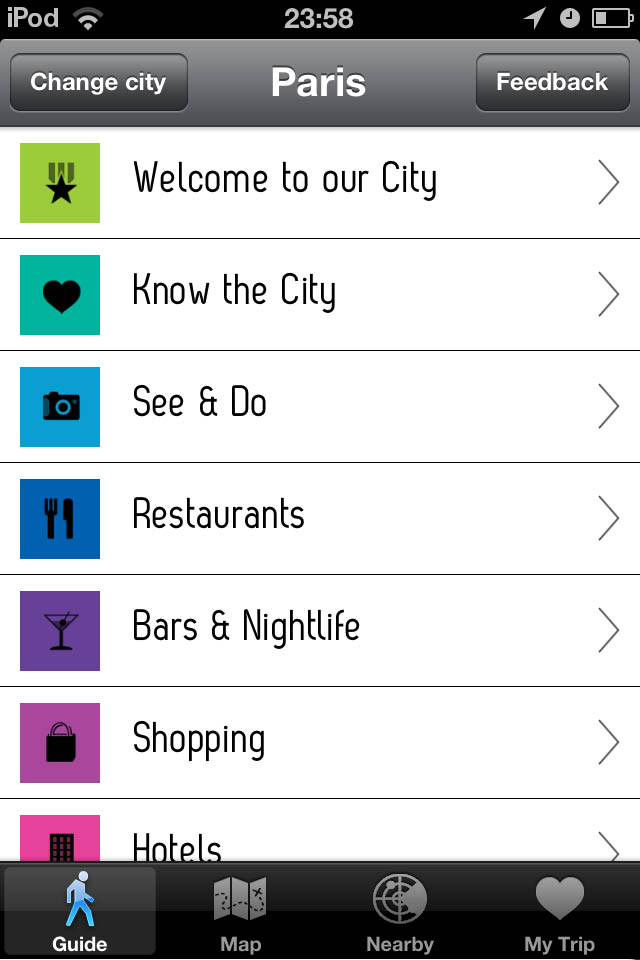
\includegraphics[height=7.5cm]{./images/screenshots/screenshot_guidepal_1.jpg}
                \caption{Category selection for filtering the locations.}
                \label{fig:guidePalCategorySelection}
        \end{subfigure}%
        \quad\quad\quad\quad\quad
        \begin{subfigure}[b]{0.25\textwidth}
                \centering
                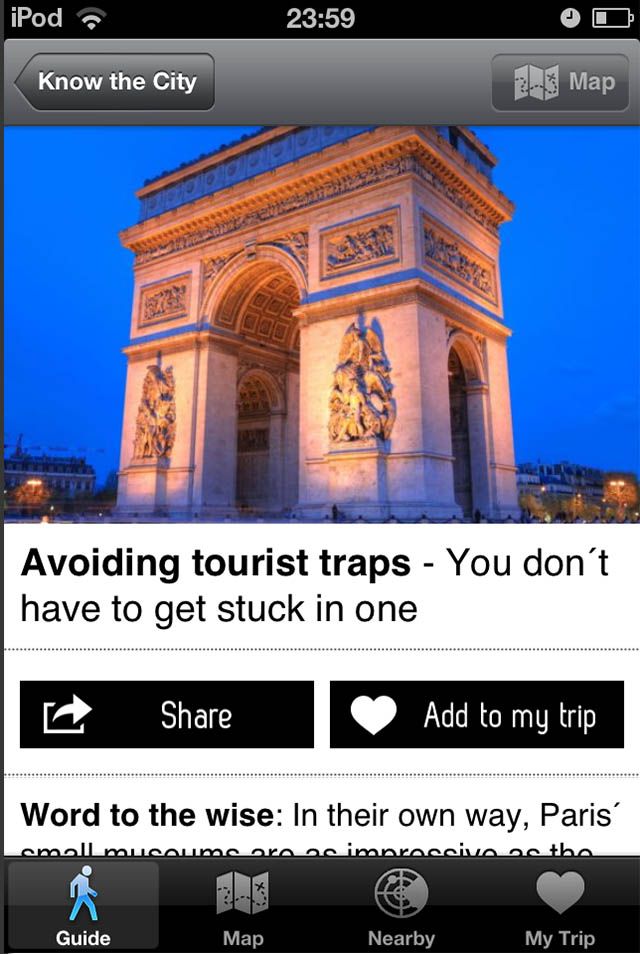
\includegraphics[height=7.5cm]{./images/screenshots/screenshot_guidepal_2.jpg}
                \caption{Detailed information about touristic location.}
                \label{fig:guidePalDetailedInformation}
        \end{subfigure}
        \caption{GuidePal~\cite{GuidePalWeb}\cite{GuidePaliPhone} iPhone application screenshots.}
        \label{fig:guidePalIphoneScreenshots}
\end{figure}
\\
In order to list the existing points of interest, the user selects the desired city and category as illustrated by  Figure~\ref{fig:guidePalIphoneScreenshots}~(\subref{fig:guidePalCategorySelection}). After selecting the intended category, a description for the point of interest is presented; Figure~\ref{fig:guidePalIphoneScreenshots}~(\subref{fig:guidePalDetailedInformation}) shows the selection of the "Know the City" category.\\
\\
This application also have some augmented reality features, providing users with the possibility to map the real world (captured by the camera of the device) with the touristic attractions in real time. When the camera points to the direction where touristic locations are available near by, those are presented above the image. By selecting any of the presented locations, the user is redirected to the detail page similar to one illustrated on Figure~\ref{fig:guidePalIphoneScreenshots}~(\subref{fig:guidePalDetailedInformation}).
%%%%%%%%
\subsection{mTrip}
mTrip~\cite{mTrip} travel guide service is mainly used for big cities such as Paris, Berlin,  Madrid, and others. It is available as a separate application for each one of the major cities (for both iPhone and Android) and allows people to consult information regarding points of interest without an Internet connection. Figure~\ref{fig:mtripScreenshots} presents some screenshots of this application. \\
\\
Users can plan an itinerary or create guides for the cities by providing the detailed information on the touristic attractions they plan to visit. After specifying the dates for the trip, each user can manually compose his itinerary or allow mTrip to automatically generate an itinerary for the trip. When the automatic mode is chosen, one must indicate preferences for the attractions to be visited, as shown on Figure~\ref{fig:mtripScreenshots}~(\subref{fig:mTripPreferencesCustomization}). A list of points of interest is presented when the user selects a specific category, similar to those shown on Figure~\ref{fig:mtripScreenshots}~(\subref{fig:mTripTouisticLocations}).
\\
%%%%%%%%%%%%%%%%%
\begin{figure}
        \centering
        \begin{subfigure}[b]{0.25\textwidth}
                \centering
                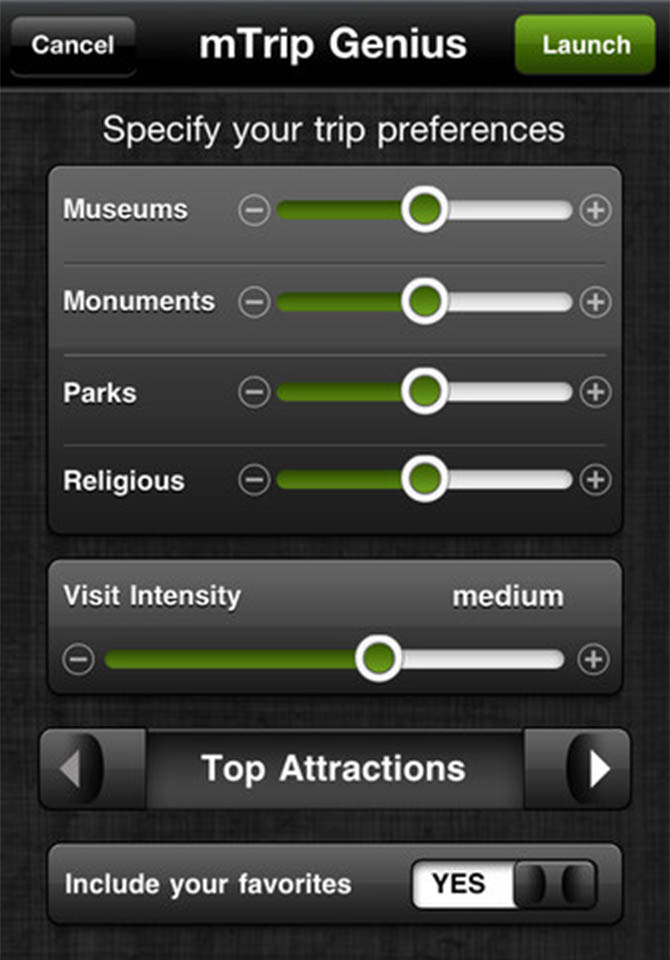
\includegraphics[height=7.5cm]{./images/screenshots/screenshot_mtrip_1.jpg}
                \caption{Customization of the itinerary.}
                \label{fig:mTripPreferencesCustomization}
        \end{subfigure}%
        \quad\quad\quad\quad\quad\quad
        \begin{subfigure}[b]{0.25\textwidth}
                \centering
                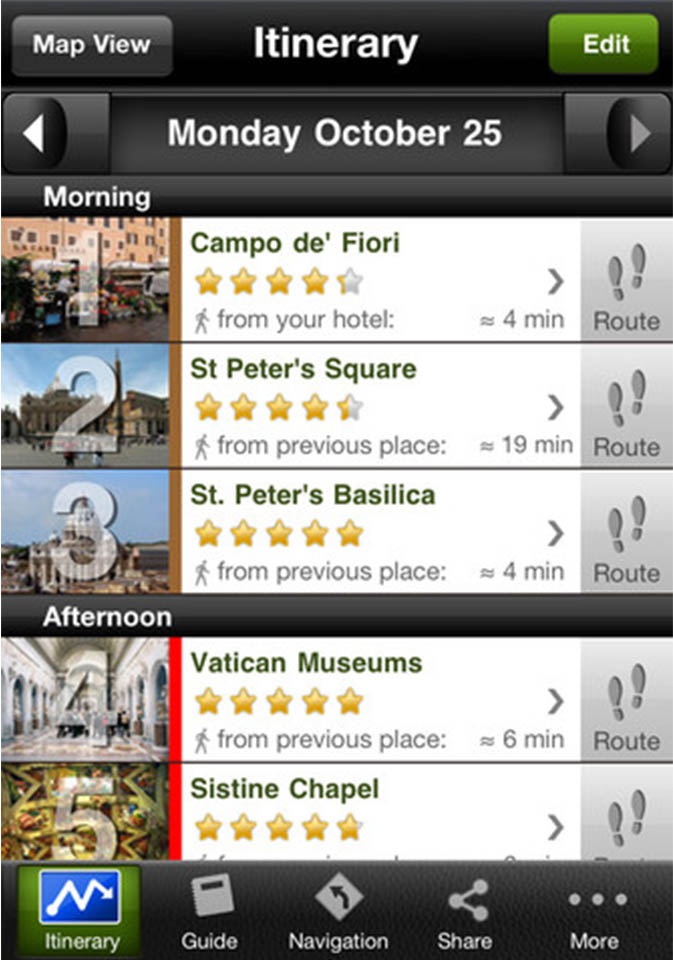
\includegraphics[height=7.5cm]{./images/screenshots/screenshot_mtrip_2.jpg}
                \caption{List of the touristic locations.}
                \label{fig:mTripTouisticLocations}
        \end{subfigure}
        \caption{mTrip iPhone application screenshots.}
        \label{fig:mtripScreenshots}
\end{figure}
\\
%%%%%%%%%%%%%%%%%
Each point of interest is accompanied by a description, a photo, opening hour, prices, as well as the comments and ratings from other travellers. The application provides an augmented reality tool that allows to preview of the points of interest around the user's current location.
%%%%%%%%
\subsection{Triposo}
Triposo~\cite{triposo} shares similar concepts with the mTrip application. However, it includes much more countries as well as smaller cities. When one picks the country to visit, the download of information regarding the points of interest for that country starts immediately, allowing to consult this information later in offline mode. Some major cities require additional downloads due to the large amount of the points of interest and touristic attractions. For big cities, users have access to special information regarding the city guide about all sights, a list of restaurants and extended nightlife options. The application also offers a travel dashboard with currency converter, weather, and useful native language phrases. Triposo uses freely available content from different sources, such as Wikipedia~\cite{wikipedia}, Wikitravel~\cite{wikitravel}, World66~\cite{world66}, among others.\\
\\
As it is shown by the screenshot on Figure~\ref{fig:triposoScreenshots}~(\subref{fig:triposoSuggestedPointsOfInterest}), a set of suggested points of interest for Lisbon is presented along with the main navigation items. Figure~\ref{fig:triposoScreenshots}~(\subref{fig:triposoWeahtherTime}) shows the current weather and current time for Porto as well as the spelling of some Portuguese words.\\
%%%%%%%%%%
\begin{figure}
        \centering
        \begin{subfigure}[b]{0.25\textwidth}
                \centering
                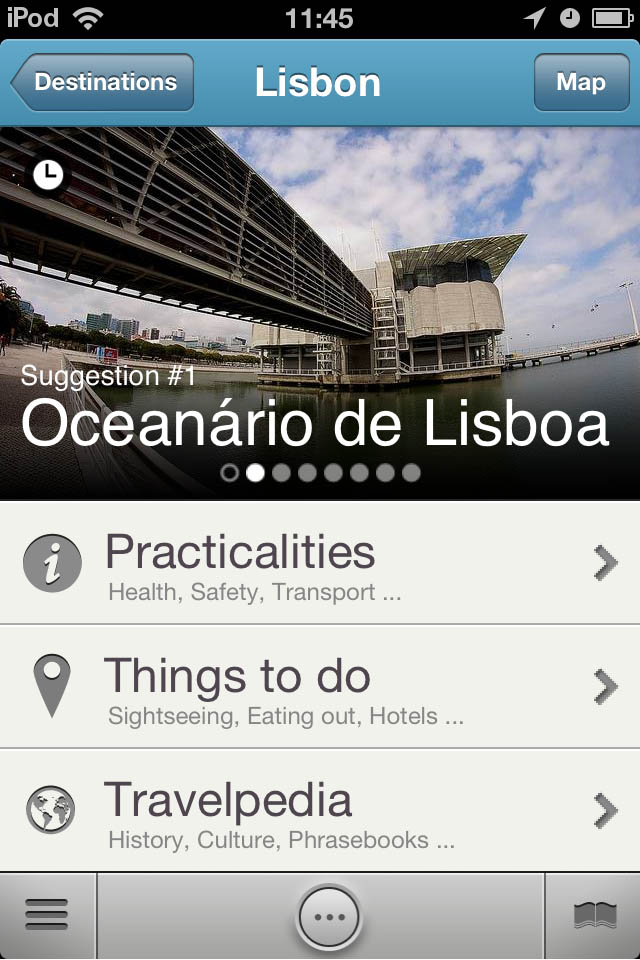
\includegraphics[height=7.5cm]{./images/screenshots/screenshot_triposo_1.jpg}
                \caption{Suggested points of interest.}
                \label{fig:triposoSuggestedPointsOfInterest}
        \end{subfigure}%
        \quad\quad\quad\quad\quad
        \begin{subfigure}[b]{0.25\textwidth}
                \centering
                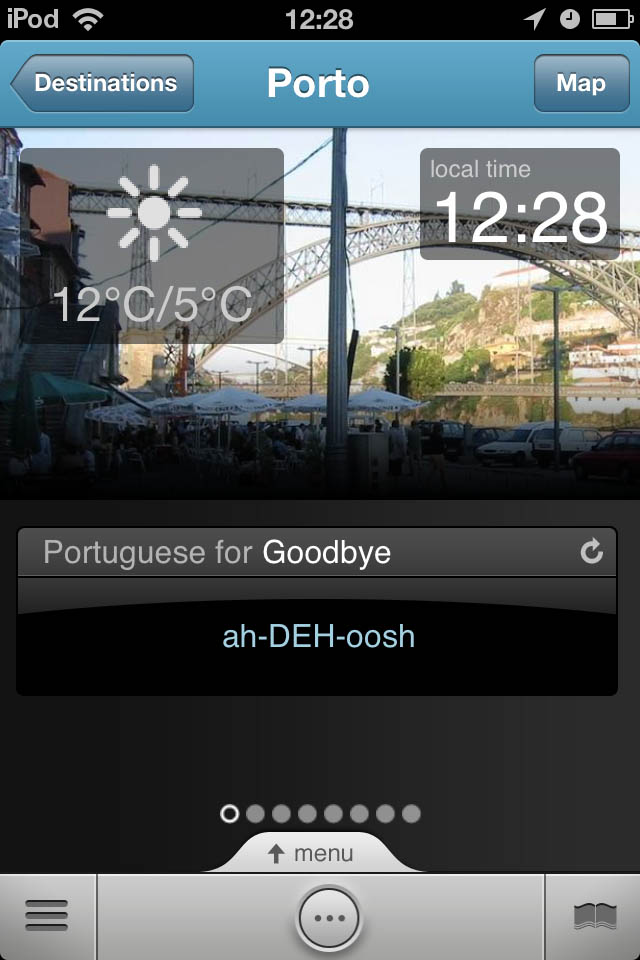
\includegraphics[height=7.5cm]{./images/screenshots/screenshot_triposo_2.jpg}
                \caption{Shortcuts and useful information.}
                \label{fig:triposoWeahtherTime}
        \end{subfigure}%
        \caption{Triposo iPhone application screenshots.}
        \label{fig:triposoScreenshots}
\end{figure}


%%%%%%%%%%
\subsection{Foursquare}
Foursquare is a service that allows registered users to "check-in\footnote{Check-in refers to the user's action for posting his current location at a venue.}" at their current location. It is composed by both web and mobile applications for iPhone, Android and Blackberry. Users with special permission have the possibility to contribute with new locations, such as coffee shops, restaurants, sights, among others. The service was created in 2009 and in March of 2011 a new version with a recommendation engine~\cite{foursqureRecommendationEngine} was developed, for suggesting places that users might like, based on their past actions.\\
\\
In 2013 an updated version of the service was launched, where users can consult the sights nearby their current location. The map view with the recommended sights nearby users current location is shown on Figure~\ref{fig:4SqureScreenshots}~(\subref{fig:4squre2}). An example of the touristic location details is shown on Figure~\ref{fig:4SqureScreenshots}~(\subref{fig:4squre3}) where user can have the preview of the location, save it to favourites, perform the check in, among others.\\
\\
\begin{figure}
        \centering
        \begin{subfigure}[b]{0.25\textwidth}
                \centering
                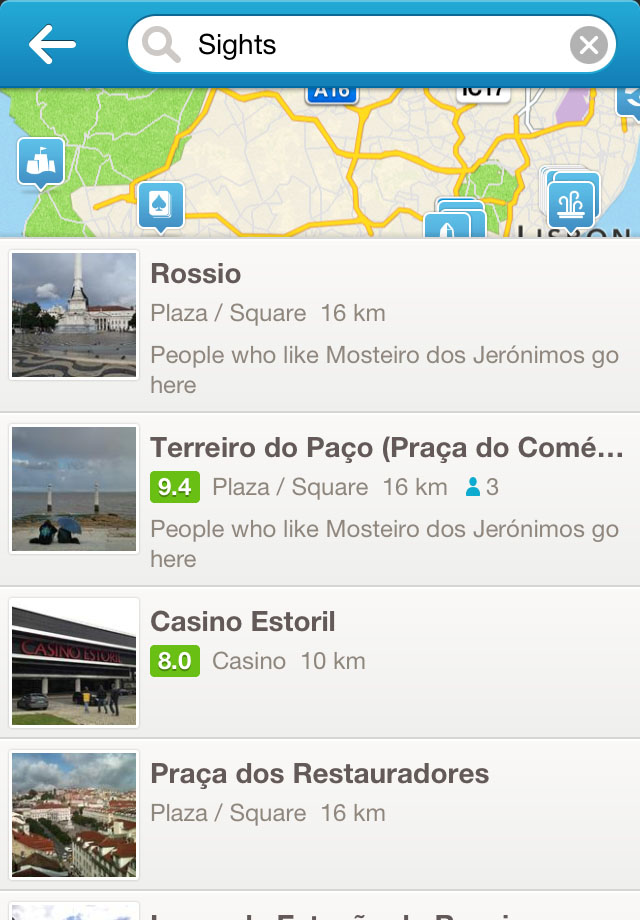
\includegraphics[height=7cm]{./images/screenshots/screenshot_foursqure_1.jpg}
                \caption{Map view with sights nearby user's location.}
                \label{fig:4squre2}
        \end{subfigure}%
        \quad\quad\quad\quad\quad
        \begin{subfigure}[b]{0.25\textwidth}
                \centering
                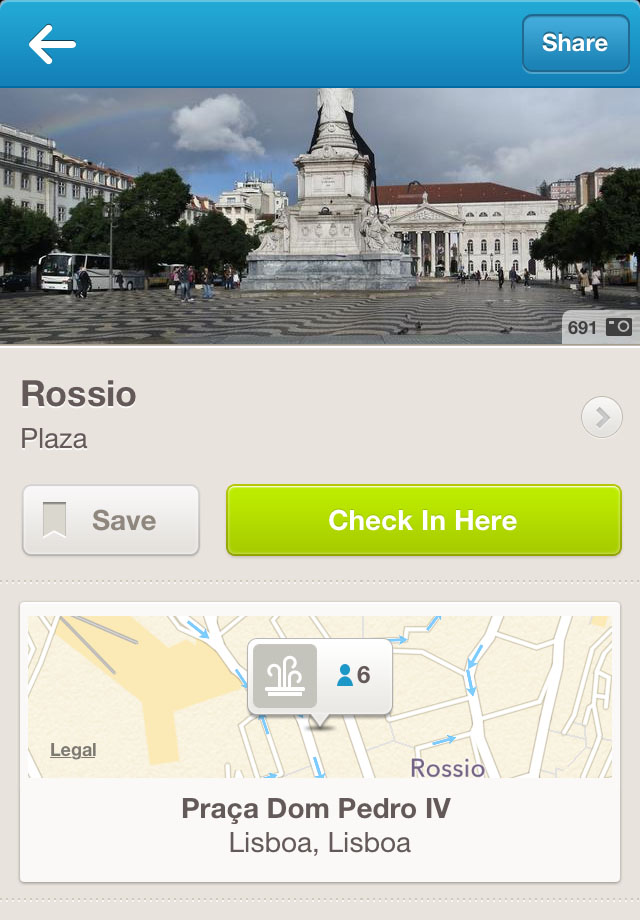
\includegraphics[height=7cm]{./images/screenshots/screenshot_foursqure_2.jpg}
                \caption{Details of the Touristic location.}
                \label{fig:4squre3}
        \end{subfigure}%
        \caption{Foursquare iPhone application screenshots.}
        \label{fig:4SqureScreenshots}
\end{figure}
\\
All these applications are modern solutions for tourist guides. The Foursquare service was created in 2009, the mTrip and TouristEye in 2010, whereas the Triposo and GuidePal have been published in 2011. 
\newpage

\section{Proposed Solution}
\label{sec:ftbd}
This Section introduces the simplified service architecture as well as the employed technologies used during the development of the system components. The system is mainly composed by the~\gls{rest}~\cite{RestWebber} service with a data access layer which exposes a set of endpoints\footnote{In \gls{soa}, an endpoint is the entry point to a service.} accessible by the client applications. Client applications are available as Web-based and Mobile (for iOS~\cite{ios} platforms iPhone and iPad). Figure~\ref{fig:introductioArchitecture} shows the proposed service architecture.\\
\\
\begin{figure}[h!]
 \centering
   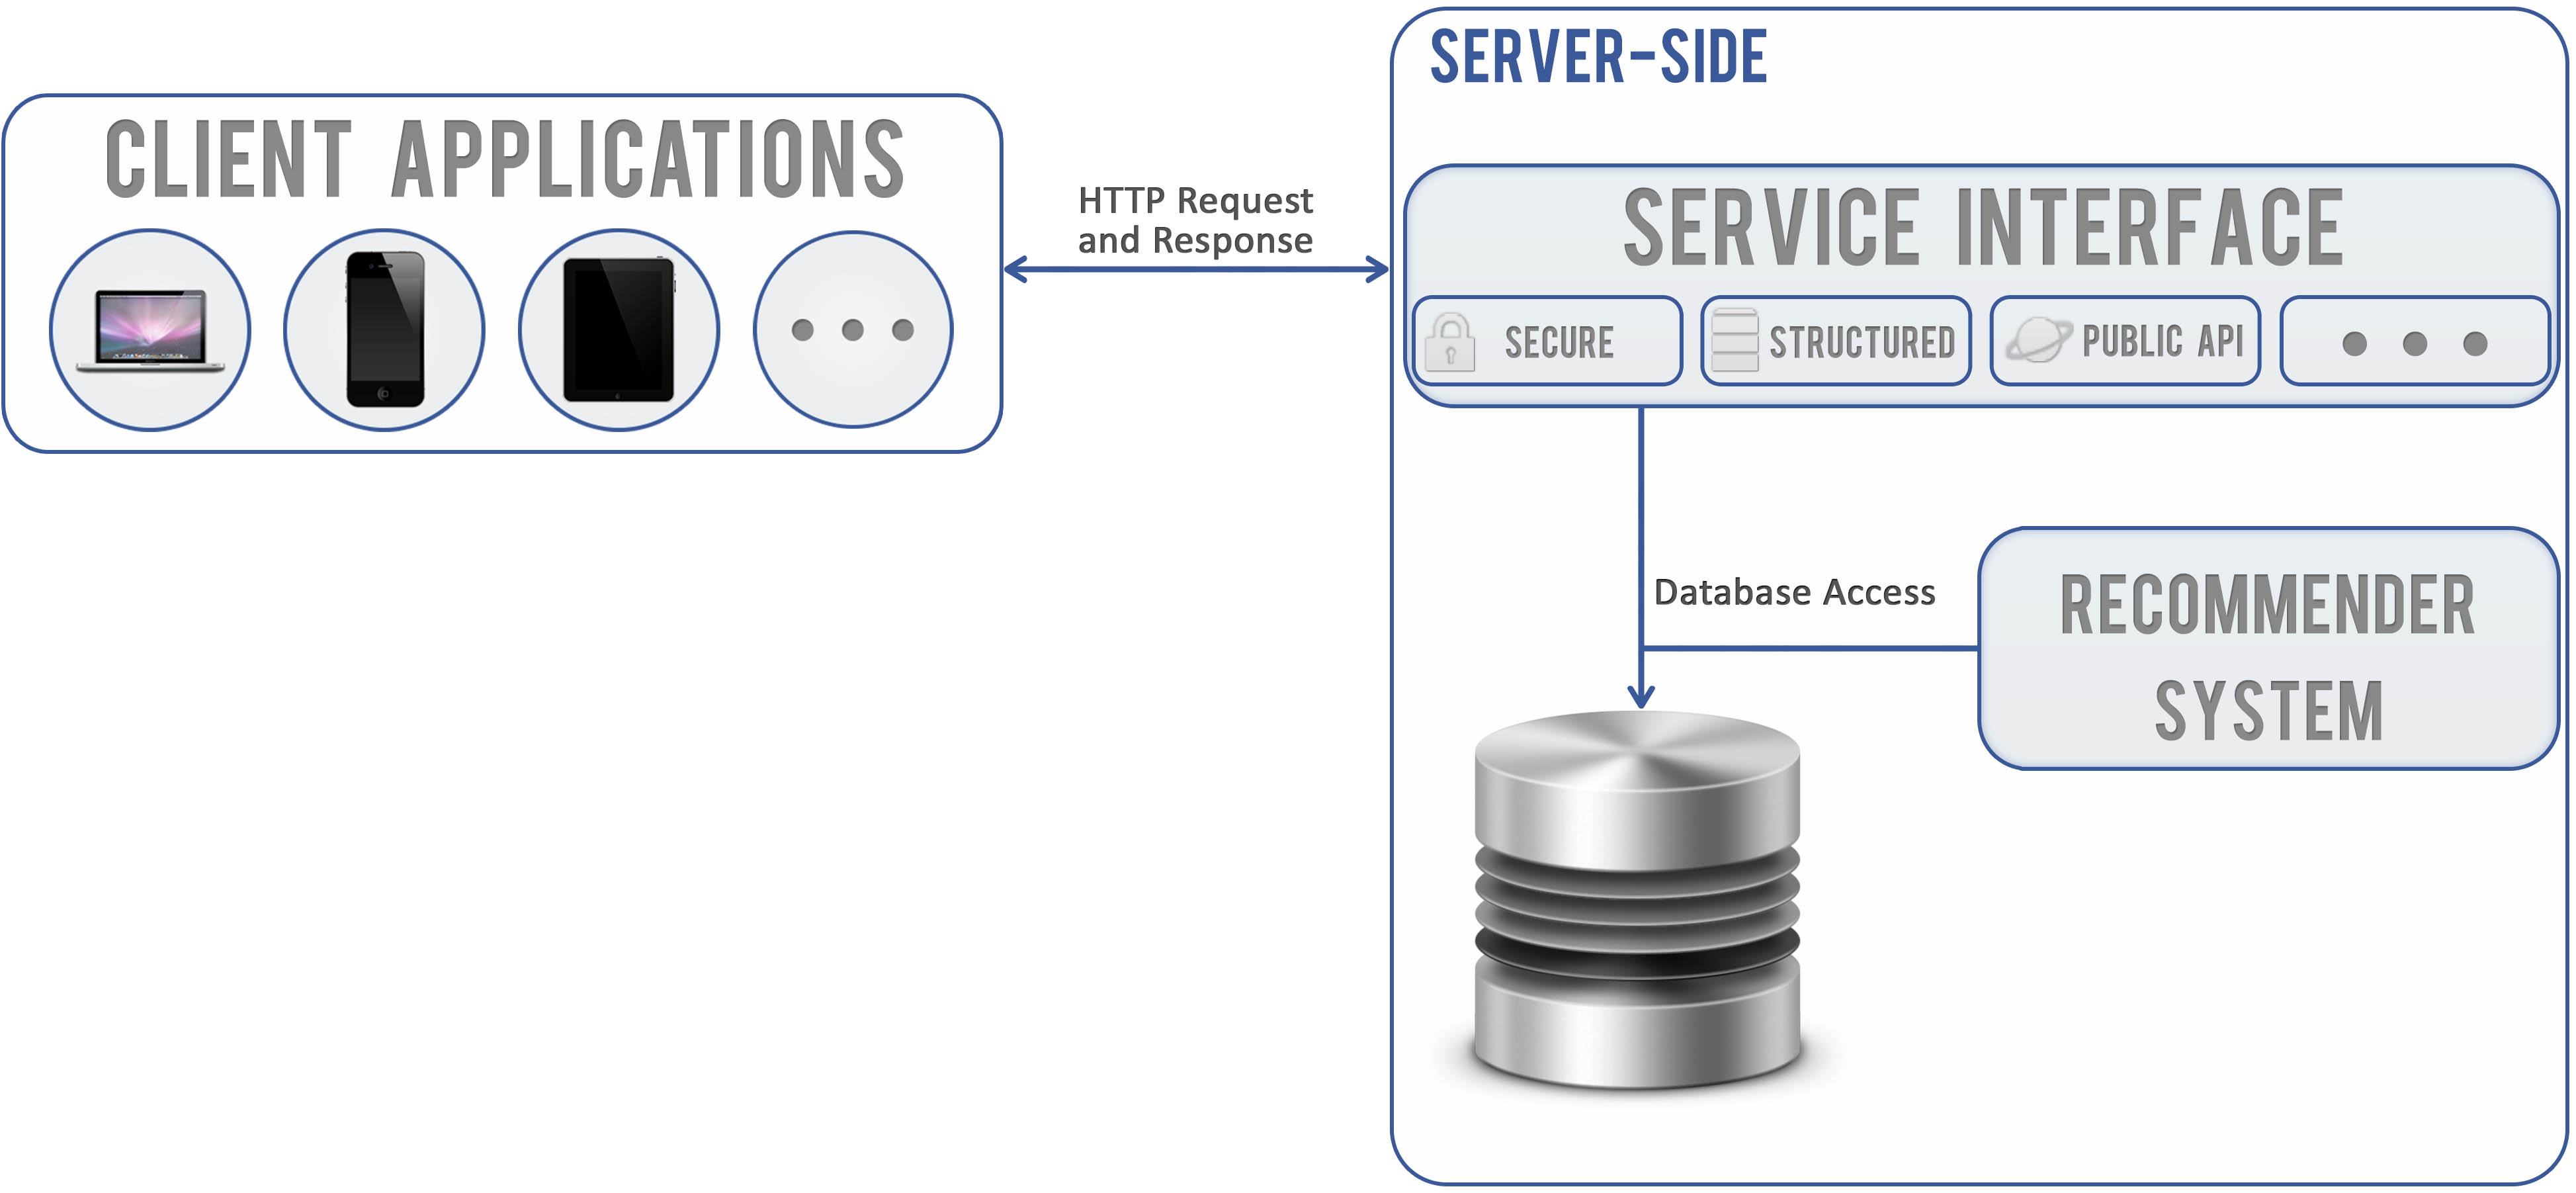
\includegraphics[width=14.8 cm]{./images/diagrams/diagram_introduction_architecture.jpg}
   \caption{Generic service architecture.}
   \label{fig:introductioArchitecture}
\end{figure}\\
\\
The service is divided into four main layers, with the following roles:
\begin{itemize}
 \item The Database layer stores information regarding points of interest, user data, among other types of data.
 \item The Service Interface is responsible for communicating with the Database layer. It makes all accesses transparent to the end client applications. This layer is mainly responsible for the data security and integrity, delivery of information in structured format, among others.
 \item The Recommender System is responsible for finding new points of interest based on the user's past actions, and to recommend these to the user. This service uses data from the database layer in order to compute recommendations.
 \item Client Applications make \gls{http} requests in order to access data from the public \gls{api}, provided by the Service Interface layer.
\end{itemize}

\subsection{Tools and Technologies}
\label{subsec:ttbuipd}
This Subsection introduces the technologies and tools used to achieve the goals of this project. We begin by describing a set of technologies related to databases, data model, and the \gls{rest} service. Then, the Web related technologies are discussed and finally we address the mobile applications.\\
\\
%%%%
For information storage, we use the MySQL~\cite{MySqlOrcale} relational database, which uses the \gls{sql} for accessing and manipulating databases. In order to facilitate the service development process, a pre-populated database was created with a few tens of points of interest.\\
\\
%%%%
The \gls{rest}~\gls{api} is developed in order to provide a single data source for client applications, including those already developed within this project and others that may appear in the future. The \gls{api} is implemented using the Java environment and Play~Framework~\cite{playFramework}.\\
\\
The Web application implementation is focused in technologies for user interface definition and structuring such as~\gls{html5}~\cite{html5},~\gls{css3}~\cite{css3} and also the JavaScript~\cite{javaScript} technology to enrich user's interactivity. The server side of the web application was developed using the Play Framework. Twitter Bootstrap~\cite{twitterBootstrap} framework was used to generate the layout with desired dynamic content, thus providing an user friendly platform.\\
\\
%\marginpar{} %%%
In the past few years, mobile devices have been used and widespread with great success, starting with Apple's iPhone launch and later with the iPad~\cite{iPadSanchez}. Both devices share the same operating system named iOS that offers a development platform for object-oriented applications. Those are written in Objective-C~\cite{ObjectiveC}\footnote{The Objective-C is a computer programming language based on C and Smalltalk. It is designed to leverage the C language with full object-oriented programming capability, through the mechanism of message passing. When in Objective-C one sends a message, its target is resolved at runtime and then it interprets the message with the receiving object~\cite{ObjectiveC}~\cite{objectiveCBook}.} using the iOS SDK (Software Development Kit). In the course of this project the targeted applications were designed taking into consideration advanced aspects of the iOS platform such as sharing code between iPhone and iPad, by means of an Universal Application~\cite{UniversalApps}.\\
\\
%\marginpar{} %%%
The development of these applications was carried out using the \gls{ide} Xcode~\cite{Xcode}.

\subsection{Core Features}
\label{subsec:cf}
This Subsection contains a description of the core features provided by the service, which are presented in Table~\ref{tab:coreFeatures}.\\
\\
\newpage
\begin{center}
    \begin{longtable}{ | p{3.5cm} | p{11.1cm} |}
    \caption{Core features of the GuideMe service.}
    \label{tab:coreFeatures}
	\\
    \hline
    \textbf{Feature Name} & \textbf{Description}\\ \hline
    \hline
    \specialcell[t]{Internationalization\\support} & 
    The aim of the project is to support points of interest of Portugal, but its architecture is designed in order to easily be expanded and to support other countries. Multilingual support is implemented for the database, REST API and application levels. \\ 
    \hline
    
    Filtering options &
    The following features are supported:
	\begin{itemize}
	\item lookup for points of interest nearby the user's current location;
	\item filtering of the locations based on the following characteristics:
	\begin{itemize}
		\item specific attraction;
		\item user's current location, by using the geographic coordinates retrieved from the mobile device;
		\item time that the user can spend;
		\item time of day of the visit;
		\item preferred weather conditions.
	\end{itemize}
	\item places that can be visited under given weather conditions such as rainy or sunny days, among others. It requires integration with the \gls{wwo} meteorology~\gls{api}, in order to advise or not the visit to the chosen user location;
	\item filtering by the maximum distance to the point of interest, based on the user's current location and mobility.
	\end{itemize}
    \\ 
    \hline
    
    \specialcell[t]{Wanted and\\already seen} &
	Users have the possibility to create a list of locations that they intend to visit as well as access the history of already visited locations. \\ 
    \hline

	\specialcell[t]{Social component} &
    	The following features are supported:
	\begin{itemize}
	\item Integration with social networks in order to encourage users to share visits with their friends;
	\item Based on the visits and mutual preferences between various users, the system recommends new places to visit that users may like. The recommendations are produced by the recommender system, using Collaborative Filtering (CF)~\cite{ibCollabrativeVSGK}\cite{AmazonRecommendGLBSJY}\cite{recommSystemPMVS} algorithms. The proposed solution is further explained in Section~\ref{sec:ocft};
	\item The service implements the social component by itself, providing the concept of the \emph{Following} and \emph{Follower} in order to establish friendship between users. Users are notified about certain actions performed by their friends.
	\end{itemize}
    \\ 
    \hline
    
    Notification system &
    Users can receive push notifications on their iOS device when someone has started to follow them. These notifications are carried out using the~\gls{apns}~\cite{apns}.\\
\hline
    
   	Login and sign up &
    Authentication and sign up through the most popular social network services, such as Facebook~\cite{FacebookLogin} and Twitter~\cite{TwitterLogin}. \\
    \hline
    
   	Back office &
    The iOS applications implements a back office system where privileged users can create or edit an existing location. They have permission to consult log information of the different service components, to analyse and correct information regarding the touristic location that were reported by other users.\\
\hline

   	Near by  &
    Preview of the sights, near by user's geographic locations. The use-case of this feature is illustrated on Figure~\ref{fig:useCaseFilterByLocation}.\\
\hline

   	Recommended touristic locations  &
	The service performs recommendation of the touristic locations to users, based on their past visits. The detailed illustration of this scenario is shown on Figure~\ref{fig:useCaseRecommendationLocation}.\\
\hline
    \end{longtable}
\end{center}
%%%%%%%%%%%%%%%%%%%%
The use-case illustrated on Figure~\ref{fig:useCaseFilterByLocation} consists in providing the user with information regarding the sights near by his/her current location.\\
%%%%%%%%%%%%%%%%%%%%
\begin{figure}[h!]
 \centering
   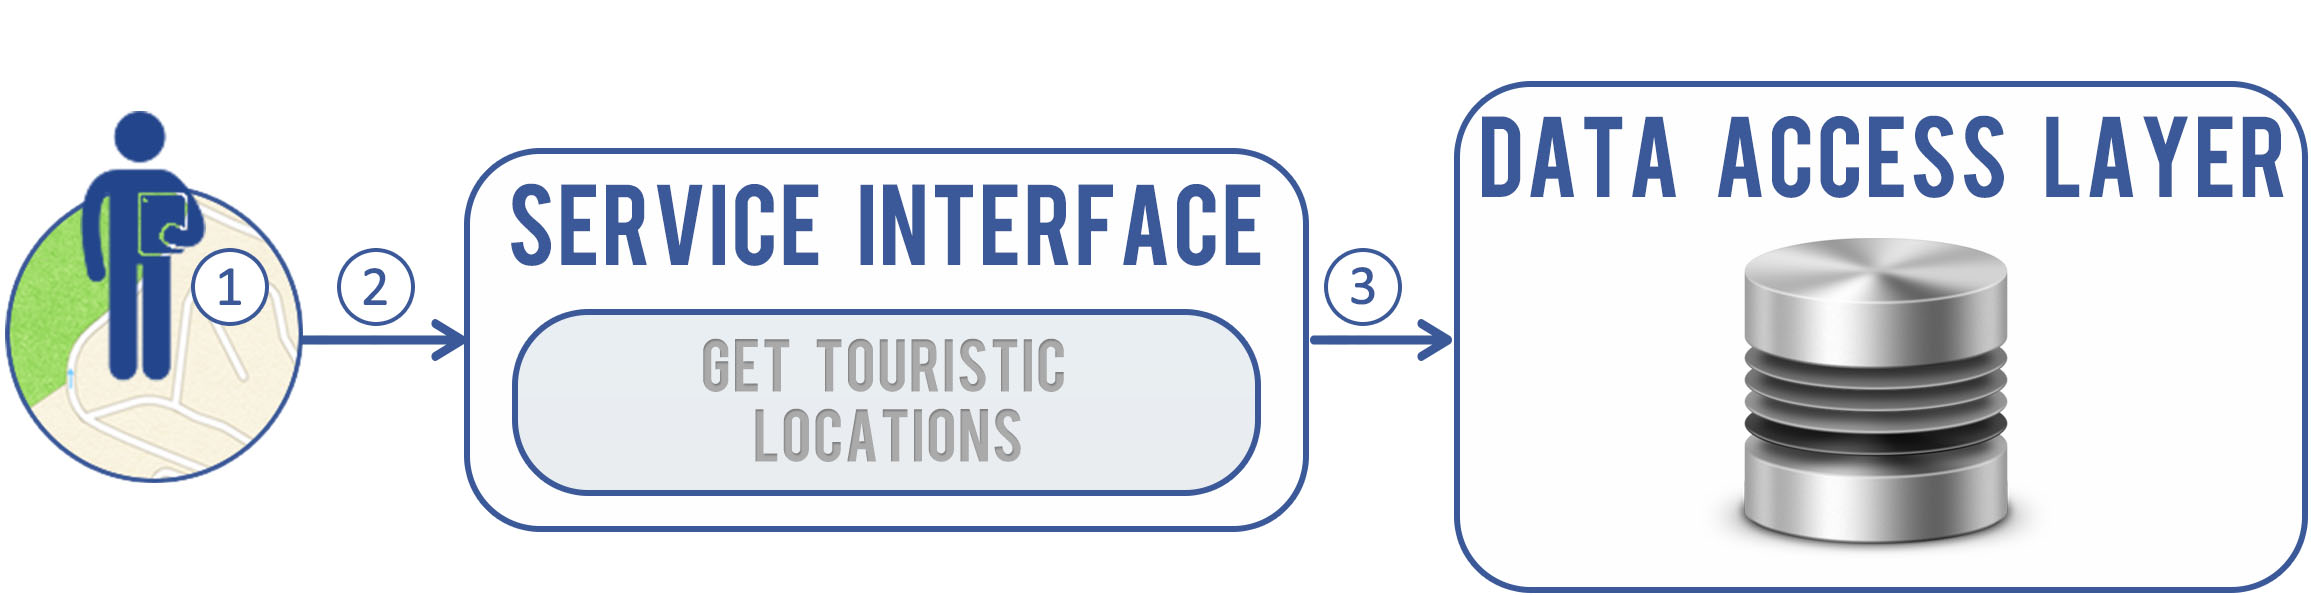
\includegraphics[width=13.0 cm]{./images/diagrams/diagram_usecase_users_location.jpg}
   \caption{Use-case of the near by feature.}
   \label{fig:useCaseFilterByLocation}
\end{figure}\\
%%%%%%%%%%%%%%%%%%%%
Each step is detailed as follows:
\begin{enumerate}
\item The geographic coordinates of user's current location, are obtained through the ~\gls{gps} of the mobile device.
\item Through the service interface, users make the requests to obtain the touristic locations passing the previously obtained geographic coordinates.
\item The service interface interacts with the Data Access Layer (DAL) in order to list the touristic locations. The distance is calculated between each sight and the submitted geographic coordinates, providing the results sorted in ascending order of distance.
\end{enumerate}
%%%%%%%%%%%%%%%%%%%%
The recommender system is one of the most important features of the developed service. The summarised process of the recommendation system is illustrated on Figure~\ref{fig:useCaseRecommendationLocation}.\\
%%%%%%%%%%%%%%%%%%%%
\begin{figure}[h!]
 \centering
   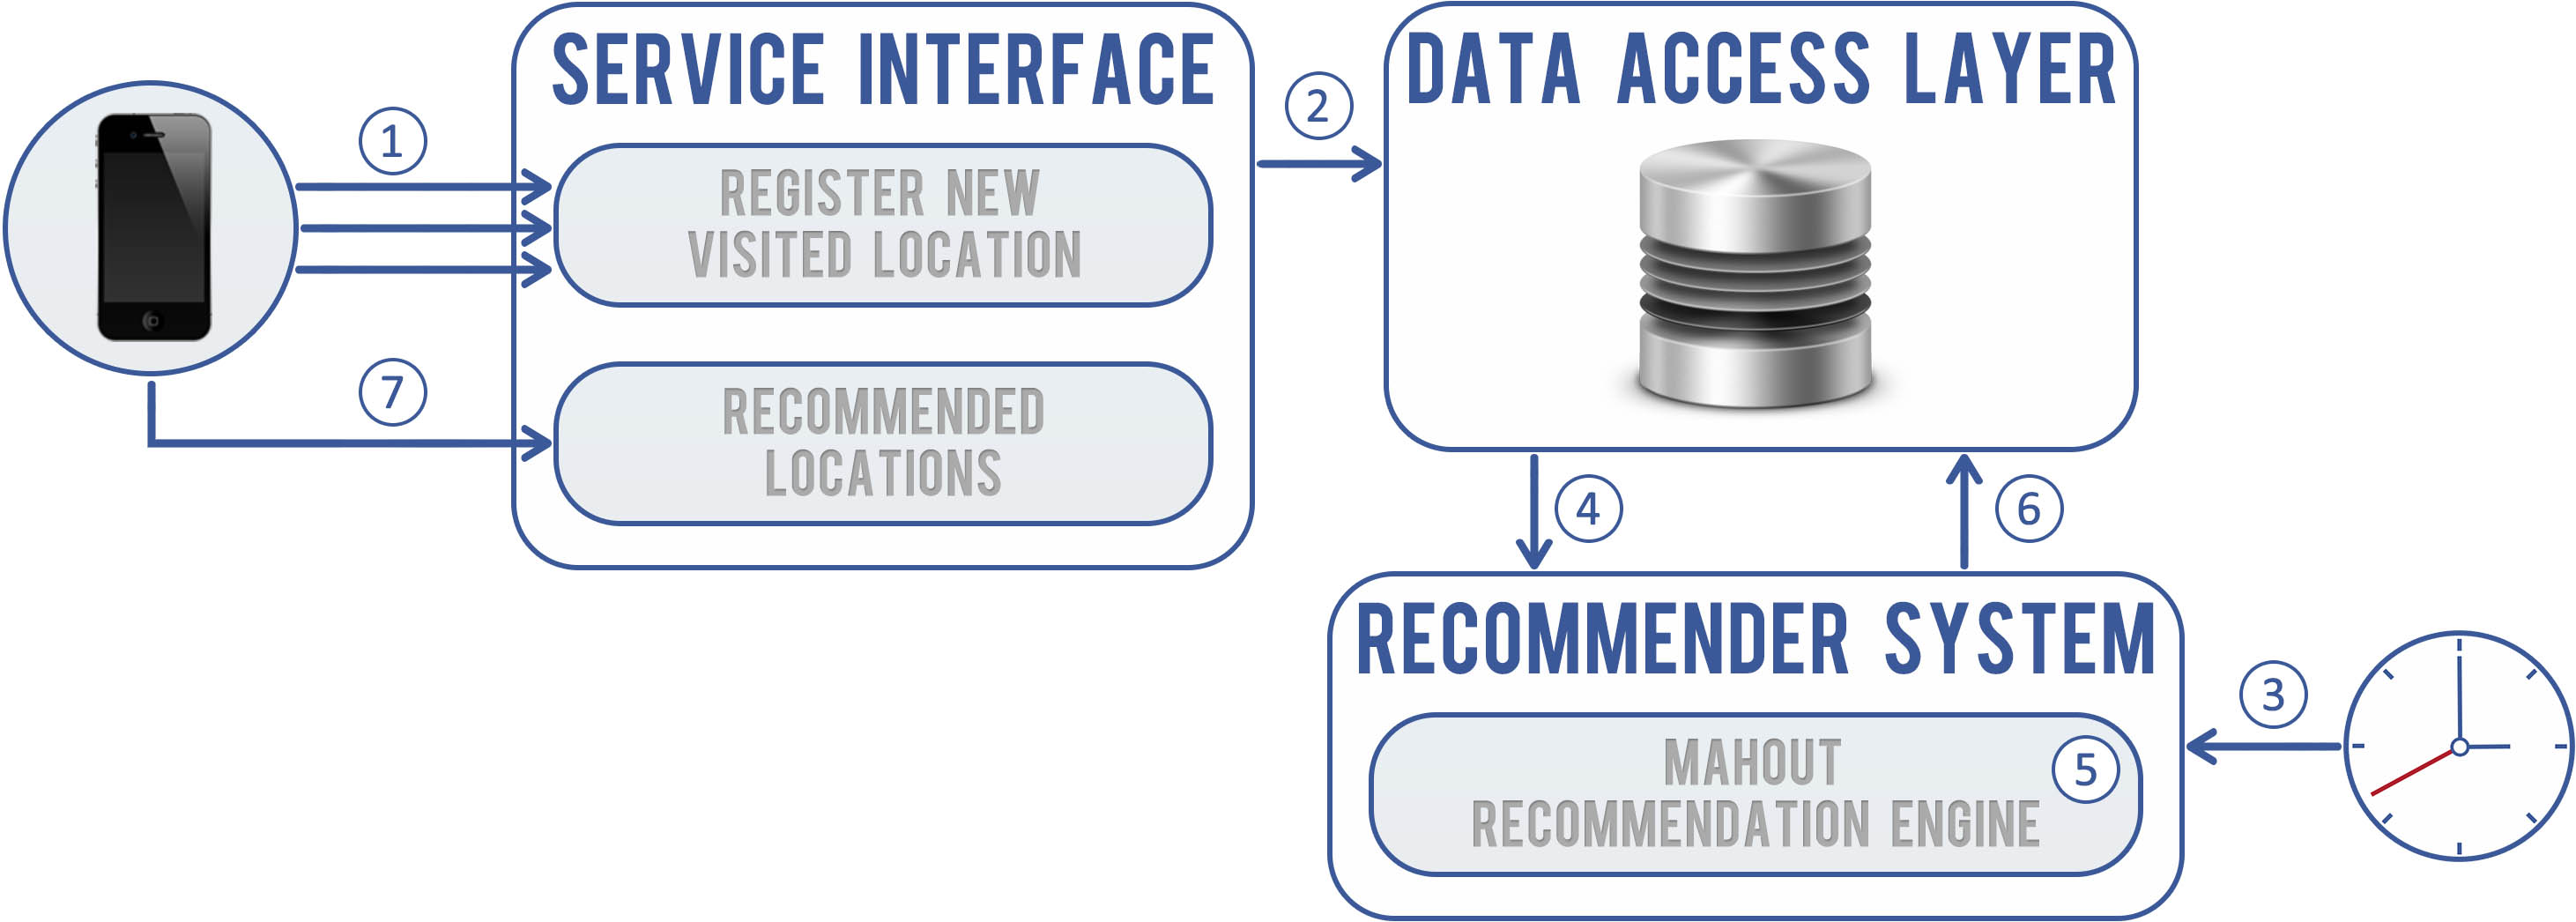
\includegraphics[width=13.0 cm]{./images/diagrams/diagram_usecase_recommender_system.jpg}
   \caption{The recommendation process.}
   \label{fig:useCaseRecommendationLocation}
\end{figure}\\
The full process of the recommendation system is as follows:
\begin{enumerate}
\item Through the service interface, the user marks new locations as visited.
\item Using the implemented DAL, the information is stored into the database.
\item The Cron Job\footnote{Cron is a time-based job scheduler in Unix-like computer operating systems.}~\cite{cronTab} is triggered everyday at 3:00 A.M., performing the recommendation process.
\item The recommender system obtains users eligible for the new recommendations.
\item For each user, the recommender system computes a set of locations previously unseen by the user.
\item Through the DAL, the recommender service removes previous recommendations and populates the database with the new information.
\item Later, the user obtains a list of recommendations through the service interface.
\end{enumerate}
%%%%%%%%%%%%%%%%%%%%
When comparing the GuideMe service with similar applications reviewed in Section~\ref{sec:sota}, it offers:
\begin{itemize}
	\item filters of unique kind that allow searching for points of interest;
	\item a friendly and usable interface for both Web and mobile applications;
	\item integration with algorithms and services that minimize human interaction during the approval process of newly inserted locations.
\end{itemize}

\section{Report Organization}
\label{sec:reportOrganization}
The remainder of this report is organized as follows. In Chapter~\ref{theory}, we introduce the background concepts and terminology of the recommender system and different collaborative filtering techniques. Chapter~\ref{implementation} approaches the proposed solution by detailing: the chosen service architecture, the integration with the~\gls{apns} service, the analysis of different frameworks for the implementation of the~\gls{dal}, and the~\gls{rest}~\gls{api}. Chapter~\ref{implementation} also includes prototypes that were initially designed before the development of the client applications.\\
\\
In Chapter~\ref{developed-work}, we describe all the developments that were made for making this project a reality. In detail, this Chapter describes the implementation aspects of the database models for both Service and Log databases, structure of the the~\gls{rest}~\gls{api} endpoints, different characteristics of the implemented recommender system, and push notification provider. We introduce the main features, as also some implementation details of the web and iOS applications. Chapter~\ref{chapter:expRsults} is devoted to the experimental results, which have guided the implementations in the correct direction. This Chapter reflects an analysis of the different recommendation system algorithms and load tests.\\
\\
We end the document with the Chapter~\ref{conclusions} by detailing the core aspects of the project and the fulfilled objectives. In order to make the service more usable and robust, as future work we present some points that should be improved in terms of security and functionalities.

\section{Our Contribution}
\label{sec:ourContribution}
We've recently submitted an article~\cite{guideMeArticle} to the 2013 Conference on Electronics, Telecommunications and Computers (CETC 2013), where we describe the main parts of this work. We believe that the developed project contribute to the evolution of tourist guide services, and promotes the effective integration of recommendation systems as a tool to easily find new interesting places to visit.
\fi

\chapter{State-of-the-Art}
\label{stateofart}
\thispagestyle{plain}

In this section, we review the state-of-the-art of the problem at hand. We start by describing why timetabling is a rather complex problem, some possible approaches to solve it and some of the existing solutions, specifically for the \gls{itc2007} benchmarks.\\

\section{Timetabling Problem}

When solving timetabling problems, it is possible to generate one of multiple types of solutions which are: \textit{feasible}, \textit{non feasible}, \textit{optimal} or \textit{sub-optimal}. A feasible solution solves all the mandatory constraints, unlike non feasible solutions. An optimal solution is the best possible feasible solution given the problem constraints. A problem may have multiple optimal solutions. Lastly, non-optimal solutions are feasible solutions that have sub-optimal values.\\
\\
Timetabling automation is a subject that has been a target of research for about 50 years. The timetabling problem may be formulated as a search or an optimization problem \cite{Schaerf1999}. As a search problem, the goal consists on finding a feasible solution that satisfies all the hard constraints, while ignoring the soft constraints. By posing the timetabling problem as an optimization problem, one seeks to minimize the violations of soft constraints while satisfying the hard constraints. Typically, the optimization is done after the use of a search procedure for finding an initial feasible solution.\\
\\
The basic examination timetabling problem, where only the \textit{clash} hard constraint is observed, reduces to the graph coloring problem~\cite{Jensen2001}, which is a well studied problem. The clash hard constraint specifies that no conflicting exams should be scheduled at the same time slot. Deciding whether a solution exists in the graph coloring problem, is a NP-complete \cite{Arora2009} problem \cite{Qu2009}. Considering the graph coloring as an optimization problem, it is proven that the task of finding the optimal solution is also a NP-Hard \cite{Arora2009} problem \cite{Qu2009}. Graph Coloring problems are explained further in Section \ref{section:existingappr}
\\
%%%%%%%%%%%%%%%%%%%%
\section{Existing Approaches}
\label{section:existingappr}
%%%%%%%%%%%%%%%%%%%%
\begin{figure}[t!]
 \centering
   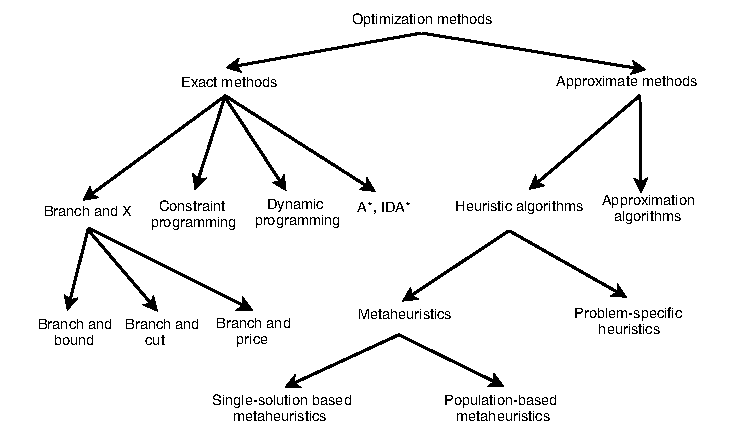
\includegraphics[width=1\textwidth,natwidth=1317,natheight=814]{./images/typesOfAlgorithms.pdf}
   \caption{Optimization methods: taxonomy and organization (adapted from \cite{Talbi2009}).}
   \label{fig:TypesAlgorithms}
\end{figure}

Figure~\ref{fig:TypesAlgorithms} depicts a taxonomy for the known optimization methods. These methods are divided into \textit{Exact methods} and \textit{Approximate methods}.\\
\\
Timetabling solution approaches are usually divided into the following categories~\cite{Qu2009}: \textit{exact algorithms} (Branch-and-Bound, Constraint Programming), \textit{graph based sequential techniques}, \textit{Single-solution based meta-heuristics} (Tabu Search, Simulated Annealing, Great Deluge), \textit{population based algorithms} (Evolutionary Algorithms, Memetic algorithms, Ant Colony algorithms, Artificial immune algorithms), \textit{Multi-criteria techniques}, \textit{Hyper-heuristics}, and \textit{Decomposition/clustering techniques}. Hybrid algorithms, which combine features of several algorithms, comprise the state-of-the-art. Due to its complexity, approaching the examination timetabling problem using exact method approaches can only be done for small size instances. Real problem instances found in practice are usually of large size, making the use of exact methods impracticable. Heuristic solution algorithms have been usually employed to solve this problem.\\
\\
Real problem instances are usually solved by applying algorithms which use both \textit{heuristics} and \textit{meta-heuristics}. Heuristic algorithms are problem-dependent, meaning that these are adapted to a specific problem in which one can take advantage of its details. Heuristics are usually used to obtain a solution (feasible or not). For example, graph-coloring heuristics are used to obtain solutions for a given timetable problem instance. Usually only the hard constraints are considered in this phase. Meta-heuristics, on the other hand, are problem-independent, and are used to optimize any type problem. In these, one usually consider both hard and soft requirements.\\
\\
Most of the existing meta-heuristic algorithms belong to one of the following three categories: One-Stage algorithms, Two-Stage algorithms and algorithms that allow relaxations~\cite{Lewis2007}. The One-Stage algorithm is used to get a solution, which the goal is to satisfy both hard and soft constraints at the same time. The Two-Stage algorithms are the most used types of approaches. This category is divided in two phases: the first phase consists in not considering the soft constraints and focusing on solving hard constraints to obtain a feasible solution; the second phase is an attempt to find the best solution, trying to solve the largest number of soft constraints as possible, given the solution of the first phase. Algorithms that allow relaxation can weaken some constraints in order to solve the \textit{relaxed problem}, while considering the satisfaction of the original constraints that were weakened, on a later stage of the algorithm.

\subsection{Exact methods}
\label{subsection:exactmethods}
Approximation algorithms like heuristics and meta-heuristics proceed to enumerate partially the search space and, for that reason, they can't guarantee finding the optimal solution. Exact approaches perform an implicit enumeration of the search space and thus guarantee that the encountered solution is optimal. A negative aspect is the time taken to find the solution. If the decision problem is very difficult (e.g., NP-Complete), in practical scenarios, given large size problem instances, it may not be possible to use this approach due to the long execution time.\\

\subsubsection{Constraint-Programming Based Technique}
The gls{cpbt} allows direct programming with constraints which gives ease and flexibility in solving problems like timetabling. Two important features about this technique are the use of backtracking and logical variables. Constraint programming is different from other types of programming, as in these types it is specified the steps that need to be executed, but in constraint programming only the properties (hard constraints) of the solution, or the properties that should not be in the solution, are specified \cite{Qu2009}.\\

\subsubsection{Integer Programming}
The \gls{ip} is a mathematical programming technique in which the optimization problem to be solved must be formulated as an Integer Problem. If the objective function and the constraints must be linear, and all problem variables are integer valued, then the \gls{ip} problem is termed \gls{ilp}. In the presence of both integer and continuous variables, then the problem is called \gls{milp}. Schaerf~\cite{Schaerf1999} surveys some approaches using the \gls{milp} technique to school, course, and examination timetabling.\\

\subsection{Graph Coloring Based Techniques}
\label{subsection:graphcoloring}
As mentioned previously, timetabling problems can be reduced to a graph coloring problem. Considering this relation between the two problems, several authors used two-phased algorithms in which graph coloring heuristics are applied in the first phase, to obtain an initial feasible solution.\\

\subsubsection{Graph Coloring Problem}
The \gls{gc} problem consists in assigning colors to an element type of a graph which must follow certain constraints. The simplest sub-type is the \textit{vertex coloring}, which the main goal is to, given a number of vertices and edges, color the vertices so that no adjacent vertices have the same color. In this case the goal is to find a solution with the lowest number of colors as possible.\\
\\
The examination timetabling problem can be transformed into a graph coloring problem as follows. The exams corresponds to vertices and there exists an edge connecting each pair of conflicting exams (exams that have students in common). With this mapping only the clash hard constraint is take into consideration. Thus, soft constraints are ignored \cite{Qu2009}.\\
\\
Given the mapping between the \gls{gc} problem and the examination timetabling problem, \gls{gc} heuristics like \textit{Saturation Degree Ordering} are very commonly used to get the initial solutions. Others like \textit{First Fit} and other \textit{Degree Based Ordering} techniques (\textit{Largest Degree Ordering}, \textit{Incidence Degree Ordering}) are also heuristic techniques for coloring graphs~\cite{Carter1996}.

%\paragraph{Saturation Degree Ordering}
%The Saturation Degree Ordering heuristic colors the vertices with more constraints first. The coloring method is as follows: while choosing a vertice to color, the ones with higher saturation degree will be colored first. The saturation degree of one vertice is the number of differently colored vertices adjacent to this vertice or, in another words, the number of different colors of all adjacent vertices. In the case of a tie, the highest saturation vertice with higher number of adjacent vertices is chosen.

\subsection{Meta-heuristics}
\label{metaheuristics}
Meta-heuristics, as mentioned above, usually provide solutions for optimization problems. In timetabling problems, meta-heuristic algorithms are used to optimize the feasible solutions provided by heuristics, like the \gls{gc} heuristics. Meta-heuristics are divided in two main sub-types, which are \textit{Single-solution meta-heuristics} and \textit{Population-based meta-heuristics}~\cite{Talbi2009}.

\subsubsection{Single-solution meta-heuristics}
Single-solution meta-heuristics main goal is to modify and to optimize one single solution, maintaining the search focused on local regions. This type of meta-heuristic is therefore exploitation oriented. Some examples of this type are \textit{\gls{sa}}, \textit{Variable-Neighborhood Search}, \textit{\gls{ts}}, and \textit{Guided Local Search}~\cite{Talbi2009}. 

\subsubsection{Population-based meta-heuristics}
Population-based meta-heuristics main goal is to modify and to optimize multiple candidate solutions, maintaining the search focused in the whole space. This type of meta-heuristic is therefore exploration oriented. Some examples of this type are \textit{Particle Swarm}, \textit{Evolutionary Algorithms}, and \textit{Genetic Algorithms}~\cite{Talbi2009}.

\subsection{ITC2007 Examination timetabling problem: some approaches}
\label{subsection:ApprITC2007}

In this section, the five \gls{itc2007} - Examination timetabling track - finalists approaches are described. This timetabling problem comprises 12 instances of different degree of complexity. Through the available website, competitors could submit their solutions for the given benchmark instances. Submitted solutions were evaluated as follows. First, it is checked if the solution is feasible and a so-called distance to the feasibility is computed. If it is feasible, the solution is further evaluated based on the fitness function, which measures the soft constraints total penalty. Then, competitors' solutions are ranked based on the distance to feasibility and solution's fitness value. The method achieving the lower distance to feasibility value is the winner. In the case of a tie, the competitor's solution with the lowest fitness value wins. A solution is considered feasible if the value of distance to feasibility is zero. The set of hard constraints is the following:
\begin{itemize}
	\item no student must be elected to be present in more than one exam at the same time;
	\item the number of students in a class must not exceed the room's capacity;
	\item exam's length must not surpass the length of the assigned time slot;
	\item exams ordering hard constraints must be followed; e.g., $Exam_1$ must be scheduled after $Exam_2$;
	\item room assignments hard constraints must be followed; e.g., 	$Exam_1$ must be scheduled in $Room_1$.
\end{itemize}

It is also necessary to compute the fitness value of the solution which is calculated as an average sum of the soft constraints penalty. The soft constraints are listed below:
\begin{itemize}
	\item two exams in a row -- a student should not be assigned to be in two adjacent exams in the same day;
	\item two exams in a day -- a student should not be assigned to be in two non adjacent exams in the same day;
	\item period spread -- the number of times a student is assigned to be in two exams that are \textit{N} time slots apart should be minimized;
	\item mixed durations -- the number of exams with different durations that occur in the same room and period should be minimized;
	\item larger exams constraints - reduce the number of large exams that occur later in the timetable;
	\item room penalty -- avoid assigning exams to rooms with penalty;
	\item period penalty -- avoid assigning exams to periods with penalty.
\end{itemize}

To get a detailed explanation on how to compute the values of fitness and distance to feasibility based on the weight of each constraint, please check the \gls{itc2007} website~\cite{McCollum2007}.\\

%The finalists are ranked based their rankings on the instances. For full details on the rankings system, please consult~\cite{McCollum2007}.\\

We now review the \gls{itc2007}'s five winners approaches. The winners list of the \gls{itc2007} competition is as follows:
\begin{itemize}
	\item 1st Place - Tom\'{a}\v{s} M\"{u}ller
	\item 2nd Place - Christos Gogos
	\item 3rd Place - Mitsunori Atsuta, Koji Nonobe, and Toshihide Ibaraki
	\item 4th Place - Geoffrey De Smet
	\item 5th Place - Nelishia Pillay
\end{itemize}
We now briefly describe these approaches.\\
\\
Tom\'{a}\v{s} M\"{u}ller's approach \cite{Mueller2009} was actually used to solve all three problems established by the \gls{itc2007} competition. He was able to win two of them and to be finalist on the third. For solving the problems, he opted for an hybrid approach, organized in a two-phase algorithm. In the first phase, Tom\'{a}\v{s} used the Iterative Forward Search (IFS) algorithm \cite{Mueller2005} to obtain feasible solutions and Conflict-based Statistics \cite{Mueller2004} to prevent IFS from looping. The second phase consists in using multiple optimization algorithms. These algorithms are applied in this order: \gls{hc} \cite{Russell2010}, \gls{gd} \cite{Dueck1993}, and optionally \gls{sa}~\cite{Kirkpatrick1983}.\\
\\
Gogos was able to reach second place in the Examination Timetabling track. Gogos' approach~\cite{Gogos2012}, like M\"{u}ller's, is a two-phase approach. The first phase starts by the application of a pre-processing stage, in which the hidden dependencies between exams are discovered in order to speed up the optimization phase. After the pre-processing stage, a construction stage takes place, using a meta-heuristic called \textit{\gls{grasp}}. In the second phase, optimization methods are applied in this order: \gls{hc}, \gls{sa}, \gls{ip} (the Branch and Bound procedure), finishing with the so-called Shaking Stage, which is only used on certain conditions. The Shaking Stage \textit{shakes} the current solution creating an equally good solution, which is given to the \gls{sa}. The objective of this stage to make \gls{sa} restart with more promising solutions and generate better results.\\
\\
Atsuta et al. ended up in third place on the Examination Timetabling track and won third and second place on the other tracks as well, with the same approach for all of them. The approach~\cite{Atsuta2007} consists on applying a constraint satisfaction problem solver adopting an hybridization of \gls{ts} and Iterated Local Search.\\
\\
Geoffrey De Smet's approach \cite{Smet2007} differs from all others because he decided not to use a known problem-specific heuristic to obtain a feasible solution, but instead used what is called the \textit{Drool's rule engine}, named \textit{drools-solver} \cite{Drools}. By definition, the drools-solver is a combination of optimization heuristics and meta-heuristics with very efficient score calculation. A solution's score is the sum of the weight of the constraints being broken. After obtaining a feasible solution, Geoffrey opted to use a local search algorithm (\gls{ts}) to improve the solutions obtained using the drools-solver.\\
\\
Nelishia Pillay opted to use a two-phase algorithm variation, using a \textit{Developmental Approach based on Cell Biology} \cite{Pillay2007}, which goal consists in forming a well-developed organism by the process of creating a cell, proceeding with cell division, cell interaction and cell migration. In this approach, each cell represents a time slot. The first phase represents the process of creating the first cell, cell division and cell interaction. The second phase represents the cell migration.

\subsection{Other approaches}
\label{subsection:OtherAppr}

Abdullah et al.'s 2009 approach \cite{Abdullah2009} consists on using an hybridization of an electromagnetic-like mechanism and the \gls{gd} algorithm. In this approach, the electromagnetism-like mechanism starts with a population of timetables randomly generated. Electromagnetic-like mechanism is a meta-heuristic algorithm using an \textit{attraction-repulsion} mechanism \cite{Javadian2008} to move the solutions the region of optimal solutions.\\
\\
McCollum et al.'s 2009 two phased approach \cite{McCollum2009} use an adaptive ordering heuristic from \cite{Burke2004}, proceeding with an \textit{extended version} of \gls{gd}. As the author stated, this approach is robust and general considering the obtained results on the benchmark datasets from \gls{itc2007}.\\
\\
Alzaqebah et al.'s 2011 two phased approach \cite{Alzaqebah2011} starts by using a graph coloring heuristic (largest degree ordering) to generate the initial solution and ends by utilizing the \textit{Artificial Bee Colony} search algorithm to optimize the solution.\\
\\
Turabieh and Abdullah's 2011 approach \cite{Turabieh2011} utilizes a two phase algorithm. The first phase consists on constructing initial solutions by using an hybridization of graph coloring heuristics (least saturation degree, largest degree first and largest enrollment). The second phase utilizes an hybridization of electromagnetic-like mechanism and \gls{gd} algorithm, just like in \cite{Abdullah2009}.\\
\\
Turabieh and Abdullah proposed another approach in 2012 \cite{Abdullah2012} that utilizes a Tabu-based memetic algorithm which consists on an hybridization of a genetic algorithm with a Tabu Search algorithm. The authors state that this approach produces some of the best results when tested on \gls{itc2007}'s datasets.\\
\\
Demeester et al. in 2012 created an hyper-heuristic approach \cite{Demeester2012}. The heuristics utilized are 'improved or equal' (equivalent to hill climbing that accepts equally good solutions), \gls{sa}, \gls{gd} and an adapted version of the \textit{late acceptance} strategy \cite{Burke2008}. These heuristics are used on already-created initial solutions. Initial solutions are constructed using an algorithm which does not guarantee the feasibility of the solution.\\
\\
McCollum et al.'s 2012 approach \cite{McCollum2012} introduce an IP formulation to the ITC 2007 instance, and also a solver using the CPLEX software.\\
\\
Sabar et al.'s utilized a graphical coloring hyper-heuristic on its approach in 2012 \cite{Sabar2012}. This hyper-heuristic is composed of four hybridizations of these four methods: last degree, saturation degree, largest colored degree and largest enrollment. This approach seems to compete with the winners' approaches from \gls{itc2007}, considering the benchmark results.\\
\\
Sabar et al.'s 2012 approach \cite{Sabar2012a} utilizes a two phase algorithm. Starts by using an hybridization of graph coloring heuristics to obtain feasible solutions and a variant of honey-bee algorithm for optimization. The hybridization is composed of least saturation degree, largest degree first, and largest enrollment first, applied in this order.\\
\\
Abdullah and Alzaqebah opted to create an hybridization approach in 2013 \cite{Abdullah2013}, mixing the utilization of a modified bees algorithm with local search algorithms (i.e. \gls{sa} and late acceptance \gls{hc}).\\
\\
Salwani Abdullah and Malek Alzaqebah in 2014 constructed an approach \cite{Alzaqebah2014} that utilizes an hybridization of a modified artificial bee colony with local search algorithm (i.e. late acceptance \gls{hc}).\\
\\
Burke et al.'s 2014 approach \cite{Burke2014} uses an hyper-heuristic with hybridization of low level heuristics (neighbor operations) to improve the solutions. The low level heuristics are \textit{move exam}, \textit{swap exam}, \textit{kempe chain move} and \textit{swap times lot}. After applying this hyper-heuristic with the hybridizations, the hybridization with the best results was tested with multiple exam ordering methods, applying another hyper-heuristic with hybridizations. The heuristics applied are \textit{largest degree}, \textit{largest weighted degree}, \textit{saturation degree}, \textit{largest penalty} and \textit{random ordering}.\\
\\
Hmer and Mouhoub's approach \cite{Mouhoub2014} uses a multi-phase hybridization of meta-heuristics. Works like the two phase algorithm but includes a pre-processing phase before the construction phase. This pre-processing phase is divided in two phases: the propagation of ordering constraints and implicit constraints discovery. The construction phase utilizes a variant of \gls{ts}. The optimization phase uses hybridization of \gls{hc}, \gls{sa} and an extended version of \gls{gd} algorithm.\\
\\
Hamilton-Bryce et al. \cite{Hamilton-Bryce2014} in 2014 opted to use a non-stochastic method on their approach \cite{Hamilton-Bryce2014} when choosing examinations in the neighborhood searching process on the optimization phase. Instead, it uses a technique to make an intelligent selection of examinations using information gathered in the construction phase. This approach is divided in 3 phases. The first phase uses a \textit{Squeaky Wheel} constructor which generates multiple initial timetables and a weighted list for each timetable generated. Only the best timetable and its weighted list is passed to the second phase. The second phase is the \textit{Directed Selection Optimization} phase which uses the weighted list created in the construction phase to influence the selection of examinations for the neighbor search process. Only the best timetable is passed onto the next phase. The third phase is the \textit{Highest Soft Constraint Optimization} phase which is similar to the previous phase but weighted list values are calculated based on the solution's individual soft constraints penalty.\\
\\
Rahman et al.'s approach \cite{Rahman2014} is a constructive one. This divides examinations in sets called \textit{easy sets} and \textit{hard sets}. Easy sets contain the examinations that are easy to schedule on a timetable and on the contrary, hard sets contain the ones that are hard to schedule and so are identified as the ones creating infeasibility. This allows to use the examinations present on the hard sets first on future construction attempts. There's also a sub-set within the easy set, called \textit{Boundary Set} which helps on the examinations' ordering and shuffling. Initial examinations' ordering  are accomplished by using graph coloring heuristics like largest degree and saturation degree heuristics.\\
\\
Rahman et al.'s approach \cite{Rahman2014a} utilizes adaptive linear combinations of graph coloring heuristics (largest degree and saturation degree) with an heuristic modifier. These adaptive linear combinations allows the attribution of difficulty scores to examinations depending on how hard their scheduling is. The ones with higher score, and so harder to schedule, are scheduled using two strategies: using single or multiple heuristics and with or without heuristic modifier. The authors conclude that multiple heuristics with heuristic modifier offers good quality solutions, and the presented adaptive linear combination is a highly effective method.\\


\begin{table}
\renewcommand\arraystretch{1.4}\arrayrulecolor{LightSteelBlue3}
\captionsetup{singlelinecheck=false, font=blue, labelfont=sc, labelsep=quad}
\caption{Timeline}\vskip -1.5ex
\begin{tabular}{@{\,}r <{\hskip 2pt} !{\foo} >{\raggedright\arraybackslash}p{15cm}}
\toprule
\addlinespace[1.5ex]
2007	& Atsuta et al. - Constraint satisfaction problem solver using an hybridization of TS and iterater local search.\\
		& Smet - drool's solver with \gls{ts}.\\
		& Pillay - Two phase approach using Developmental Approach based on Cell Biology (creating the first cell, cell division, cell iteration and cell migrations).\\
2009 	& M\"{u}ller - Two-phase approach with hybridization, which the first phase includes \gls{ifs} and Conflict-based Statistics, and the second phase is composed of \gls{hc}, \gls{gd} and \gls{sa}.\\
		& Abdullah et al. - Hybridization of electromagnetic-like mechanism and \gls{gd} algorithm.\\
		& McCollum et al. - Two phase approach, which first phase consists on using adaptive ordering heuristic, and the second phase utilizes an \textit{extended version} of \gls{gd}.\\
2011	& Alzaqebah and Abdullah - Two phase approach, which the first phase uses the largest degree ordering, and the second phase utilizes an Artificial Bee Colony search algorithm.\\
		& Turabeih and Abdullah - Two phase approach, which the first phase utilizes an hybridization of graph coloring heuristics, and the second phase uses an hybridization of electromagnetic-like mechanism and \gls{gd} algorithm.\\
2012	& Gogos - Considered a two-phase approach with a pre-processing stage for hidden dependencies. The first phase uses the \textit{greedy randomized adaptive search procedure}, and the second phase is composed of \gls{hc}, \gls{sa}, \gls{ip} with Branch and Bound, finishing with a shaking stage.\\
		& Turabieh and Abdullah - Tabu-based memetic algorithm which is an hybridization of a genetic algorithm with \gls{ts}.\\
		& Demeester et al. - Hyper-heuristic approach of 'improved or equal', \gls{sa}, \gls{gd} and late acceptance strategy applied on already created solutions.\\
		& McCollum et al. - Approach based on \gls{ip} formulation (problem was not solved.)\\
		& Sabar et al. - Graph coloring hyper-heuristic approach using last degree, saturation degree, largest colored degree and largest enrollment.\\
		& Sabar et al. - Two phase approach, which the first phase is composed of an hybridization of graph coloring heuristics and the second phase uses an honey-bee algorithm.\\
2013	& Abdullah and Alzaqebah - Hybridization approach with a modified bee algorithm and local search algorithms like SA and late acceptance \gls{hc}.\\
2014	& Abdullah and Alzaqebah - Hybridization approach with a modified artificial bee colony with local search algorithm like late acceptance \gls{hc}.\\
		& Burke et al. - Approach uses an hyper-heuristic with hybridization of low level heuristics (neighbor operations) like, thereafter uses an hyper-heuristic with hybridization of exam ordering methods.\\
		& Hmer and Mouhoub - Multi-phase hybridization of meta-heuristics. A two phase approach with pre-processing phase. First phase uses a variant of TS, and the second phase utilzies an hybridization of \gls{hc}, \gls{sa} and an extended version of \gls{gd} algorithm.\\
		& Brice et al. - Approach with three phases. First phase uses a Squeaky Wheel constructor, second phase utilizes the weighted list created in the first phase for the neighbor search process, and the third phase uses a weighted list based on the solutions' soft constraints penalty.\\
		& Rahman et al. - Constructive approach that divides examinations into easy and hard sets.\\
		& Rahman et al. - Approach utilizes adaptive linear combinations of graph coloring heuristics, like largest degree and saturation degree, with heuristic modifier.\\
		
\end{tabular}
\end{table}

\chapter{Architecture}
\label{Architecture}
\thispagestyle{plain}

In this chapter, a description of the architecture is given. The subsystems that compose the architecture are detailed. The proposed software architecture was designed taking into consideration aspects such as: code readability, extensibility, and efficiency.

\section{System Architecture}

The architecture of this project is divided in multiple layers. These are independent from one another and each of them has its unique features considering the objectives of this project. The layers presented in the project are named \textit{\gls{dl}}, \textit{\gls{dal}}, \textit{\gls{bl}}, \textit{\gls{hl}}, \textit{\gls{tl}}, and \textit{\gls{pl}}. The assortment, dependencies and the main classes of each layer can be seen in Figure \ref{fig:SystemArchitecture}.

\begin{figure}[t!]
\centering
\begin{tikzpicture}
\begin{umlpackage}[x = 4, y = 0]{Data Layer} 

\end{umlpackage}

\begin{umlpackage}[x = 0, y=-3]{Data Access Layer}
\begin{umlpackage}[x = -0.9]{Models}
\end{umlpackage}
\umlinterface[x = 3]{IRepository}{}{}
\umlclass[x = 6]{Repository}{}{}
\end{umlpackage}

\begin{umlpackage}[y=-6]{Business Layer} 
\umlclass[x = 0]{PeriodHardConstraints}{}{}
\umlclass[x = 3.5]{Solutions}{}{}
\umlclass[x = 6]{Periods}{}{}
\umlclass[x = 8.5]{ConflictMatrix}{}{}
\umlclass[x = 12]{ModelWeightings}{}{}
\umlclass[x = -0.7, y = -1.5]{Examinations}{}{}
\umlclass[x = 3, y = -1.5]{RoomHardConstraints}{}{}
\umlclass[x = 6, y = -1.5]{Rooms}{}{}
\end{umlpackage}

\begin{umlpackage}[x = -0.2, y=-10.5]{Heuristics Layer}
\umlclass[x = 0]{Simulated Annealing}{}{}
\umlclass[x = 3.7]{Graph Coloring}{}{}
\umlclass[x = -0.6, y = -1.5]{Hill Climbing}{}{}
\end{umlpackage}

\begin{umlpackage}[x = 7.5, y=-10.5]{Tools Layer}
\umlclass[x = -0.1]{NeighborSelection}{}{}
\umlclass[x = 2.55]{Loader}{}{}
\umlclass[x = 5.3]{OutputFormatting}{}{}
\umlclass[x = 0, y = -1.5]{EvaluationFunction}{}{}
\umlclass[x = 3.7, y = -1.5]{FeasibilityTester}{}{}
\end{umlpackage}

\begin{umlpackage}[x = 2.5,y = -15]{Presentation Layer}
\umlclass[x = 0]{GraphColoringTest}{}{}
\umlclass[x = 4]{SimulatedAnnealingTest}{}{}
\end{umlpackage}

\umlassoc[geometry=-|-, anchor1 = -139, anchor2 = 60]{Data Layer}{Data Access Layer}
\umlassoc[geometry=-|-, anchor1 = -37, anchor2 = 135]{Data Access Layer}{Business Layer}
\umlassoc[geometry=-|-, anchor1 = 37, anchor2 = -143]{Heuristics Layer}{Business Layer}
\umlassoc[geometry=-|-, anchor1 = 143, anchor2 = -37]{Tools Layer}{Business Layer}
\umlassoc[geometry=-|-, anchor1 = 18, anchor2 = -149]{Presentation Layer}{Tools Layer}
\umlassoc[geometry=-|-, anchor1 = 152, anchor2 = -44]{Presentation Layer}{Heuristics Layer}
\end{tikzpicture}

\caption{Overview of subsystems that compose the system architecture.} \label{fig:SystemArchitecture}
\end{figure}

\subsection{Data Layer}

The \gls{dl} is the layer where all entities are stored. The entities, which represent the different elements of a timetable, such as exam, room, or timeslot, are instantiated after reading an \gls{itc2007} benchmark file. Entities are maintained in memory and discarded after the program is finished.

\subsection{Data Access Layer}

The \gls{dal} is the layer that allow access to the data stored in the \gls{dl}. This layer provides repositories of each type of entity. The repository was implemented in a way that its signature is generic, and so can only be created with objects that implement \verb+IEntity+. This is mandatory because the generic repository's implementation uses the identification presented in \verb+IEntity+. \\
\\
The \verb+Repository+ class stores the entities in a list, with indexes corresponding to the entities identifiers. The \verb+Repository+ provides basic \gls{crud} functions to access and edit the stored entities. The signature of the entities and all the specifications of the generic repository can be seen in the Figure \ref{fig:DataAccessLayer}.\\

\begin{figure}[t!]
\centering

\begin{tikzpicture}

\begin{umlpackage}[x = 0, y=-3]{Data Access Layer}
\begin{umlpackage}[x = -0.9]{Models}
\umlinterface[x = -10, y = 0]{IEntity}{}{}
\umlinterface[x = -10, y = -5.5]{ISolution}{}{}
\umlclass[x = -10, y = -7.5]{Solution}{}{}
\umlclass[x = -8, y = -5.5]{Period}{}{}
\umlclass[x = -5.7, y = -5.5]{Examination}{}{}
\umlclass[x = -3.5, y = -5.5]{Room}{}{}
\umlclass[x = -0.5, y = -4.5]{PeriodHardConstraint}{}{}
\umlclass[x = -0.5, y = -3]{RoomHardConstraint}{}{}
\umlclass[x = -1.2, y = -1.5]{InstitutionalModelWeightings}{}{}
\end{umlpackage}
\umlinterface[x = 3, y = 0]{IRepository<T>}
{}
{
	+Insert(entity : T) : void\\
	+Delete(entity : T) : void\\
	+GetAll() : IEnumerable<T>\\
	+GetById(id : int) : T\\
	+EntryCount() : int
}
\umlclass[x = 3, y = -5]{Repository<T>}
{
	\#list : List<T>
}
{
	+Insert(entity : T) : void\\
	+Delete(entity : T) : void\\
	+GetAll() : IEnumerable<T>\\
	+GetById(id : int) : T\\
	+EntryCount() : int
}

\end{umlpackage}


\umlimpl{ISolution}{IEntity}
\umlimpl{Solution}{ISolution}
\umlimpl[geometry=|-|]{Period}{IEntity}
\umlimpl[geometry=|-|]{Examination}{IEntity}
\umlimpl[geometry=|-|]{Room}{IEntity}
\umlimpl[geometry=-|]{PeriodHardConstraint}{IEntity}
\umlimpl[geometry=-|]{RoomHardConstraint}{IEntity}
\umlimpl[geometry=-|]{InstitutionalModelWeightings}{IEntity}
\umlimpl{Repository<T>}{IRepository<T>}
\end{tikzpicture}

\caption{Overview of the DAL and the present entity types and repositories.} \label{fig:DataAccessLayer}
\end{figure}

\subsection{Business Layer}
\label{subsec:BussinessLayer}

The \gls{bl} provides access to the repositories explained above by, in each of the business classes, affording \gls{crud} functions or get/set functions, and specific functions that depend on the type of the repository. One example of these latter functions is the following. Considering the room hard constraints repository, one could invoke a method for obtaining all room hard constraints of a given type. This can be seen in the Figure \ref{fig:BusinessLayer}, which includes all the \gls{bl} classes, methods and variables. The \gls{crud} functions provided by some of the business classes simply use the \gls{crud} functions from the Repository instance, which is presented on that same business class.\\
\\
It's possible to store multiple instances of a certain type of entity, recurring to the \gls{bl} classes, which provide \verb+Repository+ functions for that objective. If that's the case, a \verb+Repository+ instance of that type of entity is used. Thus, business classes that only store one instance, do not provide \gls{crud} functions, just \textit{set} and \textit{get} functions. This makes sense, considering it only stores one instance of an entity, instead of multiple entity instances, not needing the use of a \verb+Repository+. One example of these classes is the \verb+ConflictMatrix+. \\
\\
The \verb+ConflictMatrix+ class represents the \textit{Conflict matrix}, of size equal to the number of examinations. Each matrix element $(i,j)$ contains the number of conflicts between examinations $i$ and $j$. Even though it's not an entity that implements \verb+IEntity+, it must be easily accessed in the lower layers. There's only one instance of this class because there's only one conflict matrix for each set. Each set must be loaded using the \verb+Loader+ if that set is to be tested.\\
\\
All the business classes implement the \textit{Singleton} pattern. This decision was made because it makes sense to keep only one repository of each entity since they must be populated using the Loader each time a set is tested. Another reason is to avoid passing the instances references of the business classes to all the heuristics and tools that use them, and so, the instances can be easily be accessed statically.\\

\begin{figure}[p]
\centering
\thispagestyle{empty}
\begin{tikzpicture}

\begin{umlpackage}[y=-6]{Business Layer} 
\umlclass[x = -2, y= -14]{PeriodHardConstraints}
{
	\umlstatic{\#instance : PeriodHardConstraints}\\
	-phc\_repo : IRepository<PeriodHardConstraint>
}
{
	\umlstatic{+Instance() : PeriodHardConstraints}\\
	\umlstatic{+Kill() : void}
	+Insert(phc : PeriodHardConstraint) : void\\
	+Delete(phc : PeriodHardConstraint) : void\\
	+GetAll() : IEnumerable<PeriodHardConstraint>\\
	+GetById(id : int) : PeriodHardConstraint\\
	+GetByType(type : PeriodHardConstraint.types) :\\ IEnumerable<PeriodHardConstraint>\\
	+GetByTypeWithExamId(type : PeriodHardConstraint.types, \\
	exam\_id : int) : IEnumerable<PeriodHardConstraint>\\
	+GetExamsWithChainingCoincidence(exam\_id : int) :\\ IEnumerable<int>\\
	-GetExamsWithChainingCoincidenceAux(exams : \\
	List<int>) : void
}
\umlclass[x = 5, y = -8.2]{Solutions}
{
	\umlstatic{\#instance : Solutions}\\
	-solutions\_repo : IRepository<Solution>
}
{
	\umlstatic{+Instance() : Solutions}\\
	\umlstatic{+Kill() : void}
	+Insert(solution : Solution) : void\\
	+Delete(solution : Solution) : void\\
	+GetAll() : IEnumerable<Solution>\\
	+GetById(id : int) : Solution
}

\umlclass[x = -3, y = 0]{Periods}
{
	\umlstatic{\#instance : Periods}\\
	-periods\_repo : IRepository<Period>
}
{
	\umlstatic{+Instance() : Periods}\\
	\umlstatic{+Kill() : void}\\
	+Insert(period : Period) : void\\
	+Delete(period : Period) : void\\
	+GetAll() : IEnumerable<Period>\\
	+GetById(id : int) : Period\\
	+EntryCount() : int
}

\umlclass[x = 6, y=-12]{ConflictMatrix}
{
	\umlstatic{\#instance : ConflictMatrix}\\
	-conflict\_matrix : int[,]
}
{
	\umlstatic{+Instance() : ConflictMatrix}\\
	\umlstatic{+Kill() : void}\\
	+Get() : int[,]\\
	+Set(conflict\_matrix : int[,]) : void
}

\umlclass[x = 5, y = -4.3]{ModelWeightings}
{
	\umlstatic{\#instance : ModelWeightings}\\
	-imw : InstitutionalModelWeightings
}
{
	\umlstatic{+Instance() : ModelWeightings}\\
	\umlstatic{+Kill() : void}\\
	+Get() : InstitutionalModelWeightings\\
	+Set(imw : InstitutionalModelWeightings) : void

}

\umlclass[x = 4, y = 0]{Examinations}
{
	\umlstatic{\#instance : Examinations}\\
	-examinations\_repo : IRepository<Examination>
}
{
	\umlstatic{+Instance() : Examinations}\\
	\umlstatic{+Kill() : void}\\
	+Insert(exam : Examination) : void\\
	+Delete(exam : Examination) : void\\
	+GetAll() : IEnumerable<Examination>\\
	+GetById(id : int) : Examination\\
	+EntryCount() : int
}

\umlclass[x = -3, y = -6.5]{RoomHardConstraints}
{
	\umlstatic{\#instance : RoomHardConstraints}\\
	-rhc\_repo : IRepository<RoomHardConstraint>
}
{
	\umlstatic{+Instance() : RoomHardConstraints}\\
	\umlstatic{+Kill() : void}\\
	+Insert(rhc : RoomHardConstraint) : void\\
	+Delete(rhc : RoomHardConstraint) : void\\
	+GetAll() : IEnumerable<RoomHardConstraint>\\
	+GetById(id : int) : RoomHardConstraint\\
	+EntryCount() : int\\
	+HasRoomExclusivity(exam\_id : int) : bool\\
	+GetByType(type : RoomHardConstraint.types) : \\ 					IEnumerable<RoomHardConstraint>
}

\umlclass[x = 6, y = -16.3]{Rooms}
{
	\umlstatic{\#instance : Rooms}\\
	-rooms\_repo : IRepository<Room>
}
{
	\umlstatic{+Instance() : Rooms}\\
	\umlstatic{+Kill() : void}\\
	+Insert(room : Room) : void\\
	+Delete(room : Room) : void\\
	+GetAll() : IEnumerable<Room>\\
	+GetById(id : int) : Room\\
	+EntryCount() : int\\

}
\end{umlpackage}
\end{tikzpicture}
\caption{Overview of the BL and its main classes.} \label{fig:BusinessLayer}
\end{figure}

\subsection{Tools Layer}
The \gls{tl} represents the layer that contains all the tools used by the \gls{hl} and by the lower layers, while using the \gls{bl} to access all the stored entities. These tools are named \verb+EvaluationFunction+, \verb+Loader+, \verb+NeighborSelection+, \verb+FeasibilityTester+ and \verb+OutputFormatting+.\\
\\
\verb+EvaluationFunction+ is a tool  for solution validation, and computation of solution's fitness and distance to feasibility. A solution is only valid if the examinations are all scheduled, even if the solution is not feasible. The distance to feasibility determines the number of violated hard constraints and the fitness determines the score of the solution depending on the violated soft constraints and its penalty values. The distance to feasibility is used by the \gls{gc} heuristic to guarantee that the end solution is feasible, while the fitness is used by the metaheuristics used, such as SA, to compare different solutions.\\
\\
The \verb+Loader+ loads all the information presented in a benchmark file into the repositories. This tool is the first to be run allowing the heuristics and other tools to use the entities through the repositories. More information about this tool will be given in the Section \ref{sec:Loader}.\\
\\
The \verb+NeighborSelection+ is a tool that provides functions that verify if a certain neighbor function can be applied in the current solution, if so, it returns a \verb+Neighbor+ object. A \verb+Neighbor+ object does not represent a neighbor solution, but the changes that need to be applied to the current solution if this neighbor is to be accepted. Details about this tool will be explained in the Section \ref{sec:NeighborhoodOperators}.\\
\\
The \verb+FeasibilityTester+ is a tool that provides functions, which efficiently checks if a certain examination can be placed in a certain period or room. An exam could be moved by only changing the period, the room, or both. This tool is used by both the \gls{gc} and the \gls{sa}, even though it only works if the examination to check is not yet set in the solution provided.\\
\\
The \verb+OutputFormatting+ tool is used to create the output file given the final solution. This file obeys the output file rules represented in the \gls{itc2007}'s site \cite{McCollum2007b} in order to be able to submit the solution \cite{McCollum2007c}. Submitting the solution allows to check all violated hard constraints, soft constraints, distance to feasibility and fitness values on the site's page.

\subsection{Heuristics Layer}

The \gls{hl} offers access to all the implemented heuristics. These are the \gls{gc}, \gls{sa}, and \gls{hc}. All these heuristics are used to create the best timetable possible given a limited time. Heuristics like \gls{sa} and \gls{hc} make use of neighbor solutions, and so they utilize the \verb+NeighborSelection+ tool for this effect. They also use tools like \verb+FeasibilityTester+ and \verb+EvaluationFunction+ to help build the initial solution and check the fitness while improving the current solution, respectively.\\
\\
Extensive explanation about these heuristics will be given in the Chapters \ref{sec:SolutionInit} and \ref{sec:LocalSearch}.

\subsection{Presentation Layer}

The \gls{pl}, in this phase, works mainly as a debugger to run the all the project functionalities and to check the final results. It's in this layer that all the tests are made, like checking execution timings and changing input parameters on \gls{sa} and \gls{hc} to check if better results can be achieved.\\
\\
It is planned to be implemented, in a latter  phase, another version of the presentation layer that includes the possibility of visualization of the final and best timetable generated.














\chapter{Loader and solution initialization}
\label{sec:SolutionInit}
\thispagestyle{plain}

The Loader and the solution initializer (heuristic) are the first tools used in this project. The Loader and Graph Coloring heuristic (solution initializer) will only be executed once, so the major part of the execution time will be used by the meta-heuristic(s).

\section{Loader Module}
\label{sec:Loader}

The Loader's job is to load all the information presented in the dataset files. Each set file includes information about examinations and the enrolled students, the periods, the rooms, and their penalties, as well as the period and room hard constraints, and the information about the soft constraints, named \textit{Institutional Weightings}. The presence of period and room hard constraints are optional.\\
\\
This tool not only loads all the data to its corresponding repositories, but also creates and populates the conflict matrix depending on the data obtained previously. The conflict matrix is a matrix that has the information about the conflicts of each pair of examinations.

\subsection{Analysis of benchmark data}

Figure 4.1 presents the specifications of the 12 datasets of the \gls{itc2007}. The instances presented have different degrees of complexity, that is, ease of finding a feasible solution and number of feasible solutions. Using the \gls{gc} heuristic developed (described later in Section \ref{sec:GraphColoring}), Instance 4 is the most complex one, as no feasible solution could be obtained. The high conflict matrix density, in addition to the fact there's only one room (with capacity 1200 seats), and the presence of 40 period hard constraints, help to explain the dataset complexity.\\
\\
All the specifications and benchmark data from the 12 datasets of the \gls{itc2007} timetabling problem are shown in the Table \ref{tab:ITC2007Datasets}.

\begin{table}
\centering

\sisetup{table-alignment=center,table-figures-decimal=3}

\begin{tabular}{%
	 S[table-figures-integer=6]%
     S[table-figures-integer=6]%
     S[table-figures-integer=4]%
     S[table-figures-integer=3]%
     S%
     S[table-figures-integer=3]%
    }

\toprule

       & \multicolumn{1}{c}{\#} & \multicolumn{1}{c}{\#} & \multicolumn{1}{c}{\#} & \multicolumn{1}{l}{conflict} & \multicolumn{1}{c}{\#} \\
\multicolumn{1}{c}{Set} &  \multicolumn{1}{c}{students} & \multicolumn{1}{c}{exams} & \multicolumn{1}{c}{rooms} & \multicolumn{1}{c}{matrix}   & \multicolumn{1}{c}{time}  \\
       &		   	     & 		    & 		  & \multicolumn{1}{c}{density}  &\multicolumn{1}{c}{slots}\\ 
       
\midrule

1 	 & 7891 	 & 607	& 7 	 & 0.05 	 & 54 \\
2	 & 12743 & 870	& 49 & 0.01 	 & 40 \\
3 	 & 16439 & 934	& 48 & 0.03 	 & 36 \\
4	 & 5045  & 273 	& 1 	 & 0.15 	 & 21 \\
5 	 & 9253 	 & 1018 	& 3 	 & 0.009 & 42 \\
6 	 & 7909 	 & 242 	& 8 	 & 0.06  & 16 \\
7	 & 14676	 & 1096 	& 15 & 0.02  & 80 \\
8 	 & 7718 	 & 598 	& 8 	 & 0.05 	 & 80 \\
9 	 & 655 	 & 169 	& 3  & 0.08 	 & 25 \\
10	 & 1577 	 & 214 	& 48 & 0.05 	 & 32 \\
11	 & 16439 & 934 	& 40 & 0.03 	 & 26 \\
12  & 1653 	 & 78 	& 50 & 0.18 	 & 12 \\ 

\bottomrule

\end{tabular}

\caption{Specifications of the 12 datasets of the ITC 2007 examination timetabling problem.}
\label{tab:ITC2007Datasets}

\end{table}

\subsection{Implementation}

The development of the \verb+ILoader+ tool is divided into two main parts: the loading part, which loads the dataset file into the repositories using the business layer, and the creation and population of the conflict matrix.\\
\\
The loader was implemented using the \verb+Loader+ base class, from which the \verb+LoaderTimetable+ extends. The \verb+Loader+ class implements functions to make it easier to run through a file. These two classes are depicted in Figure \ref{fig:Loaders}\\
\\
Unlike the \verb+Loader+, \verb+LoaderTimetable+ depends on the structure of the dataset files. This class will use the Loader functions to go through a dataset file, and so, populate the repositories depending on the information read by the \verb+Loader+ class. The \verb+LoaderTimetable+ offers operations like \verb+Load+ and \verb+Unload+ to load all the information in a dataset file and to empty the repositories, respectively.\\
\\
\begin{figure}[t!]
\centering
\begin{tikzpicture}
\begin{umlpackage}[x = 2, y = 0]{Tools Layer} 
\umlclass[x = -3]{Loader}
{
}
{
	+Restart() : void\\
	+NextLine() : bool\\
	+ReadNextToken() : string\\
	+ReadCurrToken() : string\\
	+ReadNextLine() : List<string>
}
\umlclass[x = 6]{LoaderTimetable}
{
	
}
{
	+Unload() : void\\
	+Load() : void\\
	-InitSolutions() : void\\
	-InitInstitutionalWeightings() : void\\
	-InitRoomHardConstraints() : void\\
	-InitPeriodHardConstraints() : void\\
	-InitRooms() : void\\
	-InitPeriods() : void\\
	-InitExaminations() : void\\
	-InitConflictMatrix() : void
}
\end{umlpackage}

\umlVHextend[anchor1 = -180, anchor2 = 0, pos stereo=1.5]{LoaderTimetable}{Loader} 
\end{tikzpicture}

\caption{Specification of Loader and LoaderTimetable tools} \label{fig:Loaders}
\end{figure}The implementation of the \verb+LoaderTimetable+ class is all about the \verb+Load+ method. This public method will be asking for new lines and reading the tokens out of it, using the \verb+Loader+ class. This procedure will take place as long as there are new lines to read. It's a pretty simple cycle that gets a new line and checks if, for example, the string ``Exams'' is contained on that line. If so, it runs \verb+InitExaminations+, if not, checks if ``Periods'' is contained on that line, and so on, until it runs out of file. The pseudo code of this method can be seen on Algorithm \ref{alg:Load}.\\
\\
\begin{algorithm}[b!]
\begin{algorithmic}
\State Read new line
\Repeat
	\State Read next token $token$
	\State \textbf{If} $token == null$ Then $break$ 
	\State \textbf{If} $token$ Contains $"Exams"$ Then $InitExaminations()$
	\State \textbf{Else If} $token$ Contains $"Periods"$ \textbf{Then} $InitPeriods()$
	\State \textbf{Else If} $token$ Contains $"Rooms"$ \textbf{Then} $InitRooms()$
	\State \textbf{Else If} $token$ Contains $"PeriodHardConstraints"$ \textbf{Then} $InitPeriodHardConstraints()$
	\State \textbf{Else If} $token$ Contains $"RoomHardConstraints"$ \textbf{Then} $InitRoomHardConstraints()$
	\State \textbf{Else If} $token$ Contains $"InstitutionalWeightings"$ \textbf{Then} $InitInstitutionalWeightings()$
	\State \textbf{Else If} Cannot read new line \textbf{Then} $break$ 
\Until Always
\State $InitSolutions()$
\State $InitConflictMatrix()$
\end{algorithmic}
\caption{LoaderTimetabling's Load method.}
\label{alg:Load}
\end{algorithm}The method \verb+InitExaminations+ reads each examination and enrolled students, and store them in a Hashmap, which stores the students as keys and the examinations which they attend as values. With this student-examinations organization, the \verb+InitConflictMatrix+ simply goes to all pairs of examinations for each student, and add a conflict in the matrix for those pair of examinations.

\section{Graph Coloring}
\label{sec:GraphColoring}

Graph Coloring is the heuristic used to generate a feasible solution. This heuristic is ran right after the loader. The implementation of this heuristic was based on M\"{u}ller's approach \cite{Mueller2009}.\\

\subsection{Implementation}

The computation of the proposed heuristic is divided into four phases. In the first phase, it starts by editing the conflict matrix, in order to add the exclusion hard constraints to the conflict matrix. This process is possible because the exclusion hard constraint is also a clash between a pair of examinations. This makes the algorithm easier to implement later on, because checking the conflict matrix for a clash between a pair of examinations now works for the student conflicts and exclusion.\\
\\
The second phase simply erases all examination coincidence hard constraints' occurrences that have student conflicts. It is mentioned in the \gls{itc2007} site \cite{McCollum2007d} that if two examinations have the examination coincidence hard constraint and yet 'clash' with each other due to student enrollment, this hard constraint is ignored.\\
\\
The third phase populates and sort the assignment lists. The assignment lists are four lists that hold the unassigned examinations. These four lists contain:
\begin{itemize}
	\item Unassigned examinations with ``room exclusivity'' hard constraint
	\item Unassigned examinations with ``after'' hard constraint
	\item Unassigned examinations with ``examination coincidence'' hard constraint
	\item All other unassigned examinations
\end{itemize}
The Largest Degree Ordering Graph Coloring heuristic is used on these four lists, and so, each list is sorted by number of students conflicts. The examination assignment is done taking the present list ordering. First all the examinations with room exclusivity are assigned, then all that have the after constraints, and finally all with examination coincidence.\\
\\
The fourth phase is the examination assignment phase (the most important phase of this heuristic). It is based on M\"{u}ller's approach \cite{Mueller2009}. It starts to assign the examinations with higher conflict, as mentioned above, using the four lists method. There are two types of assignment:
\\
\begin{itemize}
	\item Normal assignment -- If it's possible to assign the chosen examination to a period and room, a normal assignment is processed. In this type of assignment, of all the possible periods to assign, one of them is chosen randomly. It should be noted that a possible period to assign means that the examination can be assigned to that period and at least in one room on that period. After choosing the period, the same will be done to the rooms, and so, a random room will be chosen from all possible assignable rooms for that examination and period. If the current examination has to be coincident to another, and so, set to the same period as the other, the rules explained will not occur. Instead, only that period will be considered and if the period is not feasible to the current examination, the normal assignment will not take place. \\
	\item Forcing assignment -- Occurs if there are no possible periods to assign the chosen examination, because the normal assignment was not possible. A random period and room are selected and the examination will be forced to be assigned on those, unassigning all the examinations that conflict with this assignment. As the normal assignment, there are exceptions to this rule. If a coincident examination is already set, the examination to be set will be forced to be on the same period as the coincident examination, in a random room. Forcing an examination to a specific period because of a coincident examination sometimes caused infinite or very long loops in the dataset 6. Because of this, there's a chance of 25\% that the previous rule does not occur, but instead, it unassigns all coincident examinations and try to assign the current examination to a random period instead.
\end{itemize}
The Graph Coloring heuristic implementation only realize assignments and unassignments of exams examinations and checks examination clashes when forcing an assignment. The feasibility checking done to periods and rooms is are made by the tool FeasibilityTester, as mentioned in Section \ref{subsec:BussinessLayer}. The GraphColoring and FeasibilityTester classes, with all the variables and methods, can be seen in Figure \ref{fig:GraphColoring}. The algorithm of the graph coloring heuristic, which was explained in this section can be seen in Algorithm \ref{alg:GraphColoring}.\\

\begin{figure}[p!]
\centering
\begin{tikzpicture}
\begin{umlpackage}[x = 2, y = 0]{Heuristics Layer} 
\umlclass[x = 0]{GraphColoring}
{
	
	-examinations : Examinations\\
	-period\_hard\_constraints : PeriodHardConstraints\\
	-periods : Periods\\
	-room\_hard\_constraints: RoomHardConstraints\\
	-rooms : Rooms\\
	-conflict\_matrix : int[,]\\
	-solution : Solution\\
	-unassigned\_examinations\_with\_exclusive : \\ List<Examination>\\
	-unassigned\_examinations\_with\_coincidence : \\ List<Examination>\\
	-unassigned\_examinations\_with\_after : \\ List<Examination>\\
	-unassigned\_examinations : \\ List<Examination>
}
{
	+Restart() : void\\
	+NextLine() : bool\\
	+ReadNextToken() : string\\
	+ReadCurrToken() : string\\
	+ReadNextLine() : List<string>
}
\end{umlpackage}
\begin{umlpackage}[x = 2, y = 0]{Tools Layer} 
\umlclass[x = 0, y = -9]{FeasibilityTester}
{
	-examinations : Examinations\\
	-period\_hard\_constraints : PeriodHardConstraints\\
	-room\_hard\_constraints: RoomHardConstraints\\
	-rooms : Rooms\\
	-conflict\_matrix : int[,]
}
{
	+IsFeasiblePeriod(soltution : solution,\\ exam : Examination, period : Period) : bool\\
	+IsFeasibleRoom(soltution : solution,\\ exam : Examination, period : Period, room : Room) : bool\\
	+IsFeasiblePeriodRoom(soltution : solution,\\ exam : Examination, period : Period, room : Room) : bool\\
	+RoomCurrentCapacityOnPeriod(solution : Solution,\\ period : Period, room : Room)\\
}
\end{umlpackage}


\umlinclude[anchors=-90 and 90, name=uses]{GraphColoring}{FeasibilityTester} 
\end{tikzpicture}

\caption{Graph Coloring and Feasibility Tester} \label{fig:GraphColoring}
\end{figure}

%%%%%%%%%%%%%%%%%%%%

\begin{algorithm}
\begin{itemize}
\item Initial solution $solution$
\end{itemize}

\begin{algorithmic}[1]
\State Add exclusion to conflict matrix
\State Erase coincidence HC that contains conflict HC
\State Populate and sort assignment examination lists

\Repeat
	\State Get the right list to use $list$
	\State Remove last examination from $list$, $exam$
	\State \textbf{If Not} NormalAssign($solution$, $exam$) \textbf{Then} ForceAssign($solution$, $exam$)
\Until No more examinations to assign
\State  \textbf{Output:} $solution$
\end{algorithmic}
\caption{Graph Coloring algorithm.}
\label{alg:GraphColoring}
\end{algorithm}

\subsection{\textcolor{green}{Statistics}}

It is important to guarantee that the implemented heuristic is stochastic, and so, has stochastic behavior. The implemented heuristic is not considered stochastic if the results are not, in most part, different from each other. In this particular case, we need to assure that the \gls{gc} produces different results in different runs. This means that generated timetables cannot have examinations placed in the same period and room for each different run. This test was performed using a colorbar figure to check for color patters between the runs, wherein periods were represented by a different color. The figure didn't show any color patters, thus concluding that the \gls{gc} was indeed behaving stochastically.

\section{Solution Initialization Results}

As mentioned previously, the goal of the initialization procedure is not to find the best solution possible (in terms of fitness), but the find of feasible solution. Some sets are simpler than others, always getting good and stable execution times. Others can be harder, getting worse execution timings and instability. An unstable set means the results vary too much, and so some tests show very good execution times and others not so much. The Graph Coloring heuristic results on the 12 sets can be seen in Table \ref{tab:GCResults}. These results were obtained by running the heuristic, 10 times for each set, and computing the average for both fitness and execution time fields.\\
\\
\begin{table}[t]
\centering

\sisetup{table-alignment=center,table-figures-decimal=3}

\begin{tabular}{%
	 l%
     S[table-figures-integer=9]%
     S[table-figures-integer=6]%
     S[table-figures-integer=6]%
     S[table-figures-integer=6]%
     S[table-figures-integer=6]%
    }

\toprule

 & \multicolumn{1}{c}{} & \multicolumn{1}{c}{Execution} & \multicolumn{1}{c}{Standard} & \multicolumn{1}{c}{Time used} & \multicolumn{1}{c}{Time used}\\
\multicolumn{1}{c}{Set} &	 \multicolumn{1}{c}{Fitness} & \multicolumn{1}{c}{time} & \multicolumn{1}{c}{Deviation} & \multicolumn{1}{c}{in the $1_{st}$} & \multicolumn{1}{c}{in the $2_{nd}$}\\
       &		   	     &\multicolumn{1}{c}{(ms)} & \multicolumn{1}{c}{$\sigma$ (ms)} & \multicolumn{1}{c}{phase (\%)} & \multicolumn{1}{c}{phase (\%)}\\
       
\midrule

1 	 & 49028 	 & 202 & 61 & 0.09 & 99.91\\
2	 & 103907 & 250 & 2 & 0.11 & 99.89\\
3 	 & 170232 & 942 & 20 & 0.43 & 99.57\\
4	 & \text{--}  & \text{--} & \text{--} & \text{--} & \text{--}\\
5 	 & 349319 	 & 227 & 5 & 0.10 & 99.9\\
6 	 & 60857 	 & 297 & 192 & 0.13 & 99.87\\
7	 & 155708	 & 569 & 19 & 0.26 & 99.74\\
8 	 & 397868 	 & 243 & 8 & 0.11 & 99.89\\
9 	 & 15680 	 & 12 & 1 & 0.01 & 99.99\\
10	 & 121164 	 & 110 & 6 & 0.05 & 99.95\\
11	 & 260310 & 3405 & 2170 & 1.54 & 98.46\\
12	 & 11887 	 & 3690 & 1829 & 1.67 & 98.33\\ 

\bottomrule

\end{tabular}

\caption{Some of the Graph Coloring's performance features.}
\label{tab:GCResults}

\end{table}The table \ref{tab:GCResults} features many tests performed to this first phase. It features, as mentioned before, the average fitness of the solutions created for each dataset, and so the average execution time, its standard deviation, and the percentage of time used in the first and second phase of this project. The standard deviation was applied because of the instability on execution times of certain datasets when creating initial solutions, using the \gls{gc} heuristic. By checking the standard deviation, the datasets 6, 11 and 12 are unstable. The datasets 11 and 12, even thought the average execution time was 3405 and 3690, the tested values varied from 864 to 7642 and 201 to 6452, respectively.\\
\\
The allowed execution time is 221000 milliseconds for each test made to each dataset. This time was picked by the benchmark program provided by the \gls{itc2007} site \cite{McCollum2007e} when executed on the machine where all testes were performed. In the results presented on the Table \ref{tab:GCResults}, we can conclude that a very short amount of time is used on this first phase, compared to the one being used on the second phase.\\
\\
As shown in table \ref{tab:GCResults}, the heuristic could not get a feasible solution for the set 4. This problem might be present because of the presence of an infinite cycle of normal and forcing assignments, resulting in assigning and unassigning the same examinations. Different approaches were tried in order to try obtaining results for set 4. These approaches include using only one unsorted list of unassigned examinations, using all four unsorted lists, and keeping the four lists sorted but changing the priority order of their usage. Oddly, using only one unsorted list led to the best results, sometimes only leaving 20 to 30 examinations to sign, while the default approach varied between 90 and 120. Unfortunately none of the approaches were good enough to generate a feasible solution.\\
\\
One possible and probably good approach would be to order the lists by examination conflict. The difference between these conflict values and the ones presented in the conflict matrix, which is used in the default approach, is that the conflict matrix's values are the total student conflicts between one examination and all the others, while this new approach results in ordering the examination lists by the number of examinations each examination has conflicts with.
\chapter{Proposed Approach: Local Search}
\label{chap:LocalSearch}
\thispagestyle{plain}

The proposed solution consists on the use of a local search meta-heuristic(s) in order to improve the solution given by the \gls{gc} heuristic. This approach uses \gls{sa}, based on M\"{u}ller's approach \cite{Mueller2009}, followed by the use of \gls{hc}. The use of \gls{hc} is justified by the fact that \gls{sa} does not guarantee a good control of the execution time, and so the parameters are given to make it almost use all the available time, which is, as mentioned in the previous chapter, 221 seconds. The rest of the optimization is carried out by \gls{hc}, whose execution time is perfectly controllable.

\section{Simulated Annealing}
\label{sec:SimulatedAnnealing}

\gls{sa} is a single-solution meta-heuristic (section \ref{subsec:MetaHeuristics}). This meta-heuristic optimizes a solution by generating neighbor solutions which might be accepted, given an acceptance criterion. A neighbor solution is obtained by applying a movement operator (also known as neighbor operator) to the current solution, creating a new solution which is a neighbor of the current one. A neighbor operator, in this context, could be the movement of an examination to another time slot. Being a single-solution meta-heuristic, it generates a single neighbor. The neighbor operators and the acceptance criterion are the most important parts of this algorithm. Changes on one of these, may get the algorithm to behave in very different ways and end up with quite different solutions.\\
\\
The acceptance criterion will, considering the current and a neighbor solution, give the percentage of acceptance of the neighbor solution. Most of the approaches using this heuristic accept a new neighbor solution if it is \textit{better} than the current one. Otherwise, there's a chance that the neighbor solution is still accepted, depending on certain parameters. These parameters are the \textit{Temperature} (normally given as maximum and minimum temperature) and the \textit{Cooling Schedule}. By definition, the higher the temperature, the higher is the chance to accept a worse solution over the current solution. The cooling schedule, as the name suggests, is a function that lowers the temperature at a given rate. The SA algorithm finishes when the current temperature is lower or equal to the minimum temperature. The temperature should start high enough in order to be able to escape from local optima, by accepting worse solutions found during the trajectory.

\subsection{Implementation}

The \gls{sa} was implemented in a way that it is independent from the type of the cooling schedule and neighbor generator. The \verb+SimulatedAnnealing+ class is abstract and implements everything except for the neighbor generator, which is an abstract method that must be implemented in order to decide how the neighbor generator behaves. It also does not implement the evaluation function (the one that computes the fitness value of a solution or neighbor). The \verb+SimulatedAnnealingTimetable+ implements the \verb+SimulatedAnnealing+ abstract class, which implements the neighbor generator method and the evaluation function attribute. The \verb+SimulatedAnnealing+ and \verb+SimulatedAnnealingTimetable+'s methods and attributes can be seen in Figure \ref{fig:SimulatedAnnealing}.\\
\\
\begin{figure}[p]
\centering
\begin{tikzpicture}
\begin{umlpackage}[x = 2, y = 0]{Heuristics Layer} 
\umlabstract[x = 0]{SimulatedAnnealing}
{
	\umlvirt{\#evaluation\_function : IEvaluationFunction}\\
	-cooling\_schedule : ICoolingSchedule
}
{
	+Exec(solution : ISolution, TMax : double, TMin : double, loops : int, \\ type : int, minimize : bool, time\_limit : long) : ISolution\\
	+Exec2(solution : ISolution, TMax : double, TMin : double, loops : int, \\ rate : double, type : int, minimize : bool, time\_limit : long) : ISolution\\
	+ExecLinearTimer(solution : ISolution, TMax : double, TMin : double, \\ milliseconds : long, type : int, minimize : bool) : ISolution\\
	+GetSANumberEvaluations(Tmax : double, R : double, K : double, \\ TMin : double) : long\\
	\umlvirt{\#GenerateNeighbor(solution : ISolution, type : int) : INeighbor}\\
	\umlvirt{\#InitVals(type : int) : void}
}
\umlclass[x = 0, y = -9]{SimulatedAnnealingTimetable}
{
	\#evaluation\_function : IEvaluationFunction\\
	-neighbor\_selection\_timetable : NeighborSelectionTimetable\\
	+\umlstatic{type\_random : int}\\
	+\umlstatic{type\_guided1 : int}\\
	+\umlstatic{type\_guided2 : int}\\
	-room\_change : int\\
	-period\_change : int\\
	-period\_room\_change : int\\
	-room\_swap : int\\
	-period\_swap : int\\
	-period\_room\_swap : int\\
	+generated\_neighbors : int\\
	-random : Random\\
	-total\_neighbor\_operators : int
}
{
	\#GenerateNeighbor(solution : ISolution, type : int) : INeighbor\\
	\#GenerateNeighbor(solution : Solution, type : int) : INeighbor\\
	-GenerateRandomNeighbor(solution : Solution) : INeighbor\\
	-GenerateGuidedNeighbor1(solution : Solution) : INeighbor\\
	-GenerateGuidedNeighbor2(solution : Solution) : INeighbor\\
	\#InitVals(type : int) : void\\
	+EstimateTotalNumberOfNeighbors(average\_reps : int, \\ total\_time : int, solution : Solution) : long
}
\end{umlpackage}


\umlimpl[anchors=90 and -90]{SimulatedAnnealingTimetable}{SimulatedAnnealing} 
\end{tikzpicture}

\caption{Simulated Annealing classes} 
\label{fig:SimulatedAnnealing}
\end{figure}
The \verb+SimulatedAnnealing+ abstract class has the methods \verb+Exec+, \verb+Exec2+, and \verb+ExecLinearTimer+, which are all similar, but were created to test different approaches. All these methods share the same code, with the exception of the cooling schedule (the way the temperature is updated) and acceptance criterion. The pseudo code for \gls{sa} can be seen in Algorithm \ref{alg:SimulatedAnnealing}.\\
\\
The \verb+ExecLinearTimer+ has a linear cooling schedule, which is proportional to the running time, and uses the acceptance criterion
\begin{equation}
P(\delta E, T) = e^{\frac{-\delta E}{T}},
\end{equation} with T being the current temperature and $\delta$E the fitness difference between the new neighbor and current solution.\\
\\
The \verb+Exec+ method shares the same acceptance criterion but uses a geometric cooling schedule \begin{equation}
T (i+1) = T(i).r,
\end{equation}with r being the temperature decreasing rate (0 < r < 1). In the geometric cooling schedule, the closer the rate is to unity, the longer the algorithm takes to finish and wider is the area of solutions to be analyzed in the solution space.\\
\\
The \verb+Exec2+ method is the one used in this project. It uses an exponential (decreasing) cooling schedule \cite{CarvalhoLisbonNovember2004}\\
\begin{equation} 
T = T_{max}e^{-r.t},
\end{equation}
where t is the current span (counter initiated at 0), T\textsubscript{max} the maximum/initial temperature, and r the decreasing rate.\\
\\
This method also uses a different acceptance criterion \begin{equation} P(\delta E, T, f(s)) = e^{\frac{-\delta E}{T.f(s)}},
\end{equation}
being $\delta$E the fitness difference between the new neighbor and current solution, T the current temperature, and f(s) the solution fitness.
\\
\begin{algorithm}[t]
\textbf{Input:} 
\begin{itemize}
	\setlength{\itemsep}{1pt}
	\item $s$ \Comment{Initial solution}
	\item $TMax$ \Comment{Maximum temperature}
	\item $TMin$ \Comment{Minimum temperature}
	\item $loops$ \Comment{Number of loops per temperature}
\end{itemize}
\begin{algorithmic}
\State $T = Tmax$ ; \Comment{Starting temperature}
\State $Ac = AcInit()$ ; \Comment{Acceptance criterion initializer}
\Repeat
	\Repeat	
		\State Generate a random neighbor $s'$;
		\State $\delta E$ = $f(s') - f(s)$ ;
		\State \textbf{If} $\delta E \leq 0$ \textbf{Then} $s = s'$ \Comment{Accept the neighbor solution}
		\State \textbf{Else} Accept $s'$ with a probability computed using the $Ac$;
	\Until Number of iterations reach $loops$
	\State $T = g(T )$ \Comment{Temperature update}
\Until $T < TMin$
\State \textbf{Output:} $s$ \Comment{return the current (best) solution}
\end{algorithmic}
\caption{Simulated Annealing method.}
\label{alg:SimulatedAnnealing}
\end{algorithm}

\subsection{Variable Rate Computation}

As mentioned previously in Section \ref{sec:SolutionInitResults}, according to the \gls{itc2007} rules, the allowed time considering the used computer is 221000 milliseconds. As this time limit is the only imposition, it was decided to implement a \gls{sa} with an adaptive cooling schedule, in order to use all the available time for the optimization process independently of the chosen dataset. This approach contrasts with the one in which a fixed cooling schedule is used. Each set has its own characteristics and using a given set of parameters for one set does not guarantee that the results will be equivalently good for the other sets. For example, suppose that we've determined the best parameters for the first set, considering a time limit of 200000 milliseconds. Running the algorithm using the same parameters for the remaining sets will not terminate on the time limit of 200000 milliseconds: the sets with less number of resources (exams, rooms, students) will be optimized using less time; on the other way, the largest datasets will demand more time, eventually running over the imposed time limit.\\
\\
Hence, a SA with a variable rate was implemented to make this heuristic run closer to the given time limit for all the datasets. Considering it is not certain that the algorithm will run within the given 221000 milliseconds, because of its stochastic nature, a time limit was added to this meta-heuristic as well, ending this heuristic automatically if the time limit is reached. To avoid the performance degradation incurred by the algorithm's halting before reaching the end of the optimization, a time offset was imposed. This offset is a percentage of the total allowed algorithm execution time. For example, instead of letting the heuristic run for 221000 milliseconds, one allows it to run for 185640 milliseconds, to have a safety margin. The offset used is 16\%.\\
\\
In order to determine the proper cooling schedule, the algorithm starts by simulating the execution of this heuristic, by running all the neighbor operators $AverageReps$ times, which in this approach, the $AverageReps$ used is 50. Using the elapsed time and the given time limit, we estimate the number of neighbors that would be generated if this heuristic was to be run within the time limit. In order to compute the number of total neighbors, we use the expression 
\begin{equation} 
CompNeighbs = TotalTime / CompTime * AverageReps * TotalOperats,
\end{equation} being $TotalTime$ the time limit (221000 milliseconds), $CompTime$ the elapsed time used in the simulation, $AverageReps$ the number of loops that all the neighbors must run (50 runs), and $TotalOperats$ the total number of used operators (5 operators). After that, we compute the exact number of the neighbors ($TotalNeighbs$) that will be generated for the given parameters, using the default rate. This is achieved by simulating this heuristic using those parameters, cooling the current temperature until it reaches the minimum and returning the number of desired generated neighbors. If the $TotalNeighbs$ is above the $CompNeighbs$, a lower rate will be used to make another simulation, until the $TotalNeighbs$ for the given rate reaches a value that is close to the $TotalNeighbs$. The pseudo code of this method can be seen in Algorithm \ref{alg:RateComputing}.\\
\\
\begin{algorithm}[t!]
\textbf{Input:} 
\begin{itemize}
	\setlength{\itemsep}{1pt}
	\item $s$ \Comment{Solution}
	\item $TMax$ \Comment{Maximum temperature}
	\item $TMin$ \Comment{Minimum temperature}
	\item $reps$ \Comment{Number of loops per temperature}
	\item $exec\_time$ \Comment{Execution time limit}
\end{itemize}
\begin{algorithmic}
\State $sa = SAInit()$ ;
\State $n = 50$ ; \Comment{Number of times each operator runs}
\State $comp\_neighbors = sa.EstimateNumberNeighbors(n, exec\_time, s)$ ;
\State $rate = 1.50^{-02}$ ;\Comment{Initial default rate}
\State $power = -3$ ;
\State $rate\_to\_sub = 10^{power}$ ;\Comment{Rate decrementing}
\State $total\_neighbors = sa.GetNumberNeighbors(TMax, rate, reps, TMin)$ ;
\Repeat	
	\State \textbf{If} $rate - rate\_to\_sub \leq 0$ \textbf{Then} $power = power - 1$ ; $rate\_to\_sub = 10^{power}$ ;
	\State $rate = rate - rate\_to\_sub$ ;
	\State $total\_neighbors = sa.GetNumberNeighbors(TMax, rate, reps, TMin)$ ;
\Until $total\_neighbors < comp\_neighbors$
\State $rate = rate + rate\_to\_sub$ ; \Comment{To guarantee that total\_neighbors < comp\_neighbors}
\State \textbf{Output:} $rate$ \Comment{Return computed rate}
\end{algorithmic}
\caption{Rate computing.}
\label{alg:RateComputing}
\end{algorithm}Some testings were made in order to check this heuristic's behavior, using the following parameters: \textit{TMax} = 0.1, \textit{TMin} = $1e-06$, \textit{loops} = 5, \textit{exec\_time} = 50000, and the computed\_rate = 0.00016. As can be seen in Figure \ref{fig:SimulatedAnnealingPlot}, it starts by accepting all worse and better neighbor solutions. In the end, the temperature is so low that it becomes harder to accept worse solutions, ending up acting similar to the \gls{hc} procedure. The axis of abscissas represents the indexes of the generated neighbors and the axis of ordinates represents the current solution's score.\\
\\
\begin{figure}[!t]
\centering

\begin{tikzpicture}
\begin{axis}[
    title={},
    xlabel={Neighbor index},
    ylabel={Solution score},
    mark size=0.2pt
]

\addplot plot file [
    color=blue,
    mark=*,
    mark options={solid},
   	smooth
    ] {sa_plot_data.dat};

\end{axis}
\end{tikzpicture}

\caption{Simulated Annealing results} 
\label{fig:SimulatedAnnealingPlot}
\end{figure}

\section{Hill Climbing}
\label{sec:HillClimbing}

\gls{hc} is a meta-heuristic different from the \gls{sa} family of meta-heuristics, in the sense that it only accepts better solutions. So, as long as it reaches a local optimum, it can't get out of that point because each neighbor solution is worse. In this way, \gls{hc} only has one parameter that is the number of iterations or time limit, which controls the algorithm's execution time.\\
\\
In the evaluation undertaken, the best results were obtained with the \verb+Exec2+ version of \gls{sa}. \gls{sa} was parametrized in order to finish execution within the specified time limit imposed by the \gls{itc2007} rules. \gls{hc} is executed after \gls{sa}, using the remaining time, until the time limit is reached.

\subsection{Implementation}
The implementation of this heuristic is very similar to that of the \gls{sa}; it contains the classes \verb+HillClimbing+ and \verb+HillClimbingTimetable+, which are simplified versions of the \gls{sa} classes. The \verb+HillClimbing+ and \verb+HillClimbingTimetable+'s methods and attributes can be seen in Figure \ref{fig:HillClimbing}.\\
\\
\begin{figure}[t!]
\centering
\begin{tikzpicture}
\begin{umlpackage}[x = 2, y = 0]{Heuristics Layer} 
\umlabstract[x = 0]{HillClimbing}
{
	\umlvirt{\#evaluation\_function : IEvaluationFunction}\\
}
{
	+Exec(solution : ISolution, milliseconds : long, type : int, \\ minimize : bool) : ISolution\\
	\umlvirt{\#GenerateNeighbor(solution : ISolution, type : int) : INeighbor}
}
\umlclass[x = 0, y = -5]{HillClimbingTimetable}
{
	\#evaluation\_function : IEvaluationFunction\\
	-neighbor\_selection\_timetable : NeighborSelectionTimetable\\
	+\umlstatic{type\_random : int}\\
	-random : Random\\
	+generated\_neighbors : int\\
	-total\_neighbor\_operators : int\\
}
{
	\#GenerateNeighbor(solution : ISolution, type : int) : INeighbor\\
	\#GenerateNeighbor(solution : Solution, type : int) : INeighbor\\
	-GenerateRandomNeighbor(solution : Solution) : INeighbor\\
}
\end{umlpackage}


\umlimpl[anchors=90 and -90]{HillClimbingTimetable}{HillClimbing} 
\end{tikzpicture}

\caption{Hill Climbing classes} 
\label{fig:HillClimbing}
\end{figure}

\section{Neighborhood Operators}
\label{sec:NeighborhoodOperators}

Neighborhood operators are applied to a solution, in order to create other valid solutions (neighbor solutions), but not necessarily feasible. In this context, the core of all operations are the relocation of the examinations.\\
\\
The implementation of neighborhood selection went through different approaches. Firstly, random selection was implemented. This approach always chooses a random operator to generate a new neighbor. Thereafter, guided approaches were implemented. The first one raised the probability of selecting one operator if this one generated a better neighbor solution. The probability of that operator is reduced in an equal amount if the operator generated a worse solution.\\
\\
The authors have implemented other variations of the first approach, where increasingly higher/lower probabilities of neighbor selection were defined based on the success/failure of the operator. Despite this, the random approach almost always showed better results compared to the guided approaches.\\
\\
The neighborhood operators, in this context, are all based on moving examinations in terms of period or room. This implementation uses six different neighborhood operators:
\\
\begin{itemize}
	\item \textit{Room Change} - An examination is randomly selected. After that, a room is randomly selected. If the assignment of the random examination to the random room, while maintaining the period, does not violate any hard constraints, that neighbor is returned. If not, the adjacent rooms are checked until one of them yields a feasible solution. If it reaches the limit of rooms and no feasible solution is found, no neighbor is returned;\\
	
	\item \textit{Period Change} - An examination is randomly selected. After that, a period is randomly selected. If the assignment of the examination to the period, while keeping the room, does not clash with any hard constraints, that neighbor is returned. If not, the adjacent periods are sequentially checked until one of them creates a feasible solution. If it reaches the limit of periods and no feasible solution is found, no neighbor is returned;\\
	
	\item \textit{Period \& Room Change} - An examination is randomly selected. After that, a room and period are randomly selected. If the assignment of the examination to the room and period does not clash with any hard constraints, that neighbor is returned. If not, the adjacent rooms are checked for each of the next periods, until one of them creates a feasible solution. If it reaches the limit of periods and rooms and no feasible solution is found, no neighbor is returned;\\
	
	\item \textit{Room Swap} - An examination is randomly selected. After that, a room is randomly selected. If the selected examination can be placed in that room, while keeping the period, then a \textit{Room Change} neighbor is returned instead. If not, if the swapping of the examination with any of the examinations presented in the room, keeping the same period, does not clash with any hard constraints, that neighbor is returned. If not, the examinations presented in the adjacent rooms are checked until a feasible solution is found (always checking first if a \textit{Room Change} can be returned instead). If it reaches the limit of rooms and no feasible solution is found, no neighbor is returned;\\
	
	\item \textit{Period Swap} -  An examination is randomly selected. After that, a period is randonly selected. If the selected examination can be placed in that period, while maintaining the room, then a \textit{Period Change} neighbor is returned instead. If not, if the swapping of the random examination with any of the examinations presented in the period, keeping the same room, does not clash with any hard constraints, that neighbor is returned. If not, the examinations presented in the adjacent periods are tested until a feasible solution is found (always testing first if a \textit{Period Change} can be returned instead). If it reaches the limit of periods and no feasible solution is found, no neighbor is returned;\\
	
	\item \textit{Period \& Room Swap} - An examination is randomly selected. After that, a period and room are randomly selected. If the selected examination can be placed in that period and room, then a \textit{Period \& Room Change} neighbor is returned instead. If not, if the swapping of the random examination with any of the examinations presented in the period and room does not clash with any hard constraints, that neighbor is returned. If not, the examinations presented in the adjacent periods and rooms are tested until a feasible solution is found (always testing first if a \textit{Period \& Room Change} can be returned instead). If it reaches the limit of periods and rooms and no feasible solution is found, no neighbor is returned.
\end{itemize}

\subsection{Implementation}

The original concept of neighbor solution is to have another solution apart from the current one, which is the result of applying the neighborhood operator to the current solution. In order to have an efficient implementation, the neighbor only keeps the changes introduced in the solution, and not the changed solution itself. With this design, there's no need to replicate the original solution and to apply the neighborhood operator to it in order to obtain the neighbor solution. The process of replacing the original solution with the neighbor, consists in applying to the current solution the movement registered in the neighbor.\\
\\
Every neighbor object must implement the interface \verb+INeighbor+, which exposes the methods \verb+Accept+, \verb+Reverse+ and a real value that represents the fitness of the neighbor (the fitness of the new solution if this neighbor is to be accepted). The \verb+Accept+ method  moves the current solution to the neighbor solution. The \verb+Reverse+ method undoes the operation, getting then back the old solution. The different neighbors and their methods are illustrated in Figure \ref{fig:Neighbors}.\\
\begin{figure}[p!]
\centering
\begin{tikzpicture}
\begin{umlpackage}[x = 2, y = 0]{Heuristics Layer} 

\umlclass[x = 0, y = 0]{SimulatedAnnealingTimetable}{}{}
\umlclass[x = 0, y = -4]{NeighborSelectionTimetable}
{
	-examinations : Examinations\\
	-rooms : Rooms\\
	-periods : Periods\\
	-feasibility\_tester : FeasibilityTester\\
	-evaluation\_function\_timetable : EvaluationFunctionTimetable\\
}
{
	+RoomSwap(solution : Solution) : INeighbor\\
	+PeriodSwap(solution : Solution) : INeighbor\\
	+PeriodRoomSwap(solution : Solution) : INeighbor\\
	+RoomChange(solution : Solution) : INeighbor\\
	+PeriodChange(solution : Solution) : INeighbor\\
	+PeriodRoomChange(solution : Solution) : INeighbor\\
}
\umlclass[x = 0, y = -9]{INeighbor}
{
	+fitness : int\\
}
{
	+Accept() : ISolution\\
	+Reverse() : ISolution
}
\umlclass[x = -3, y = -11]{PeriodChangeNeighbor}{}{}
\umlclass[x = -3, y = -13]{RoomChangeNeighbor}{}{}
\umlclass[x = -3, y = -15]{PeriodRoomChangeNeighbor}{}{}
\umlclass[x = 3, y = -11]{PeriodSwapNeighbor}{}{}
\umlclass[x = 3, y = -13]{RoomSwapNeighbor}{}{}
\umlclass[x = 3, y = -15]{PeriodRoomSwapNeighbor}{}{}


\end{umlpackage}



\umlimpl[geometry=-|, anchors=180 and -90]{PeriodChangeNeighbor}{INeighbor} 
\umlimpl[geometry=-|, anchors=180 and -90]{RoomChangeNeighbor}{INeighbor} 
\umlimpl[geometry=-|, anchors=180 and -90]{PeriodRoomChangeNeighbor}{INeighbor} 
\umlimpl[geometry=-|, anchors=-180 and -90]{PeriodSwapNeighbor}{INeighbor} 
\umlimpl[geometry=-|, anchors=-180 and -90]{RoomSwapNeighbor}{INeighbor} 
\umlimpl[geometry=-|, anchors=-180 and -90]{PeriodRoomSwapNeighbor}{INeighbor}
\umlinclude[anchors=-90 and 90, name=uses]{SimulatedAnnealingTimetable}{NeighborSelectionTimetable}
\umlinclude[anchors=-90 and 90, name=uses]{NeighborSelectionTimetable}{INeighbor} 
\end{tikzpicture}

\caption{Neighborhood selection and operators} 
\label{fig:Neighbors}
\end{figure}

\subsection{Statistics}
\label{sub:SAStatistics}
It is important to make sure that the algorithm works as planned. This includes the desired stochastic behavior, and all the neighbor operators must contribute positively to obtain better results.\\
\\
In this particular case, to make sure this heuristic is stochastic, we must guarantee that all the examinations are moved roughly the same number of times. Considering that some examinations are harder to move, these are moved less times than others, but the difference is not significant. A study was made to compare, in the same run, the number of rejected and accepted neighbors for each examination. The examinations are sorted in descending order by the number of conflicts. Figure \ref{fig:AvsRNeighbors} represents a color map in which the colors represent the number of times each examination was accepted (x = 1) and rejected (x = 2), for set 1. As can be seen, some examinations are not even selected to move, and so, have zero accepted and rejected results. In this particular set, only two lines have zero counters, as checked in the results file. These two examinations have \textit{exam\_coincidence} hard constraint and are only able to be in one room due to the number of students being too high. The \gls{sa} algorithm is not optimized to move more than one examination at the same time. This means that those two examinations can never be moved to another period, because the \gls{sa} can only move one examination at a time and these examinations can't be moved to another room, because they don't fit in other rooms.\\
\\
Other blue lines, which have values between 1000 and 1, are rare. This occurs not only because the examination is hard to move due to its conflicts, but may also have the \textit{exam\_coincidence} and a really short number of rooms in which that examination can fit. This problem creates a limitation in the \gls{sa} heuristic, preventing the \gls{sa} from scanning parts of the solution space, and eventually degrading the quality of the final result.\\
\\
\begin{figure}[t!]
\centering

\begin{tikzpicture}

	\begin{axis}[
		colorbar style={
		scaled y ticks = false,
		y tick label style={/pgf/number format/fixed,
			/pgf/number format/1000 sep = \thinspace 	% Optional if you want to
														% replace comma as the 1000
														% separator 
        }
		},
		width = \textwidth,
		xlabel = {Accepted (x=1) and rejected (x=2) neighbors},
		ylabel = {Exam indexes},
		enlarge x limits = true,	% The value true enlarges the lower 
									% and upper limit.
									% The value false uses tight axis limits
		enlarge y limits = true,
		colorbar,
		%colormap={}{ gray(0cm)=(1); gray(1cm)=(0);}, % Grey colorbar
		%x dir = reverse,
		y dir = reverse,
		%xmode = log,        % logarithmic x axis
		%xmin = 0, xmax = 9,
		% car92 has 543 exams
		%ymin = 0, ymax = 606, 
%		ytick = { 0, 100, 200, 300, 400, 500, 542},
		extra x ticks = {
1,
2,
3
}, extra x tick labels = {},
	    		extra tick style = { grid = major},
	    		width = \textwidth,
	    		%width = 17cm,
			%height = 11cm,
		]
		\addplot[surf, 
			shader = interp, % No facets
			point meta = explicit] 
			%table [z expr = 100, meta index = 2] {./yor83Cool1Eminus6.dat};
			table [z expr = 100, meta index = 2] {./SAResults6.dat};
\end{axis}

\end{tikzpicture}

\caption{Accepted and rejected neighbors for each examination in the Simulated Annealing.}
\label{fig:AvsRNeighbors} 
\end{figure}
\subsection{Neighborhood Operators Effect}
One of the most important aspects when dealing with the \gls{sa} is the choice of the neighbor operators. It is crucial that all the neighbor operators contribute positively. If a neighbor operator contributes negatively, it's better not to use it. M\"{u}ller proposed the first five operators~\cite{Mueller2009} \textit{Room Change}, \textit{Period Change}, \textit{Period \& Room Change}, \textit{Room Swap}, and \textit{Period Swap}. We add to the M\"{u}ller's set a sixth operator, the \textit{Period \& Room Swap} operator. In the sequel we present a study of the influence of this operator. For all 12 datasets, 20 runs were performed, computing the fitness average for each of the two cases. Table \ref{tab:NeighborsImprovementFactor} shows the improvement factor for using six neighbors instead of five. In most cases, it's worse compared to using the original five neighbor operators, and so, the 6th operator will not be used in this project's results. The results of using five operators also showed that more neighbors were generated and the percentage of feasible generated neighbors compared to the unfeasible, for each dataset, is also higher compared to using six neighbor operators.

\begin{table}[!t]
\centering
\caption{Improvement factor (percentage) between using five and six neighbor operators.}
\sisetup{table-alignment=center,detect-weight=true,detect-inline-weight=math}
\begin{tabular}{%
	S[table-figures-integer=3]%
	S[table-format=5.1]%
	S[table-format=5.1]%
	S[table-format=5.1]%
		S[table-format=5.1]%
    }

\toprule

\multicolumn{1}{c}{} & \multicolumn{1}{c}{5} &	\multicolumn{1}{c}{6} &	\multicolumn{1}{c}{Improvement}\\
\multicolumn{1}{c}{Dataset} & \multicolumn{1}{c}{Neighbors} &	\multicolumn{1}{c}{Neighbor}&	\multicolumn{1}{c}{Factor (\%)}\\
\multicolumn{1}{c}{} & \multicolumn{1}{c}{Operators} &	\multicolumn{1}{c}{Operators}&	\multicolumn{1}{c}{}\\
\midrule

1   &   5019  & 5055 & \textcolor{red}{-0.7}\\
2   &   478  & 523 & \textcolor{red}{-9.4} \\
3   &   14997  & 15228 & \textcolor{red}{-1.5} \\
4   &   \text{--}  & \text{--} & \text{--}\\
5   &   4950 & 4819 & \textcolor{green}{+1.5}\\
6   &   27680  & 27528 & \textcolor{green}{+0.5} \\
7   &   4799  & 4812 & \textcolor{red}{-0.3} \\
8   &   8551  & 8741 & \textcolor{red}{-2.2} \\
9   &   1141  & 1150 & \textcolor{red}{-0.8} \\
10  &   28219  & 25586 & \textcolor{green}{+9.3} \\
11  &   45344  & 45630 & \textcolor{red}{-0.6} \\
12  &   7222  & 7679 & \textcolor{red}{-6.3} \\

\bottomrule
$\sum$  &  148400   & 146751 & \textcolor{red}{-10.5}
\end{tabular}
\label{tab:NeighborsImprovementFactor}
\end{table}


\section{Fitness Computation}
\label{sec:FitnessComputation}

Fitness evaluation in timetable automation, due to its complexity, has a great influence in the algorithm performance. Hence, good performance of this step is required. As mentioned in the Subsection \ref{subsec:ToolsLayer}, this value is computed using the \verb+EvaluationFunction+ tool, which in a first approach, implies for generated neighbors, the recalculation of their fitness value. Tests were made to study this approach since the fitness results were not as good as expected. The tests showed that this approach was having poor performance, since most of the time was used to compute the fitness for each new neighbor generated solution.\\
\\
A new approach was implemented, which consists in computing the fitness incrementally. This means that for each new generated neighbor, a new fitness value is computed based on the current solution's fitness. This approach takes advantage of the fact that the operations applied to the current solution are simple and so the neighbor solutions are, in most part, equal to the current solution. Thus, the fitness computation is performed considering only the small changes between the current solution and the new generated neighbor solution.\\
\\
Tests were made to compare both approaches and, using the same parameters, for the first set it was possible to achieve equivalent results, 19 times faster. As a consequence if both approaches would use both the same parameters, and execution time, the new approach would have generated 19 times more neighbors, thus exploring the solution space with more detail.

\subsection{Implementation}

In order to compute the fitness of the neighbor solutions incrementally, a fitness function must be implemented depending on the type of neighbor. Considering that all neighbors have a reference to the solution they derive from, and the methods \verb+Accept+ and \verb+Reject+, it's possible to access the current solution and the neighbor generated solution (\verb+Accept+ will change the current solution and so the reference presented in this neighbor, replacing with the neighbor solution). \\
\\
The differences between the fitness values of the current solution and the new neighbor's depend on the type of neighbor created. For example, if a \verb+RoomSwapNeighbor+ is created, the changes will occur in the mixed durations constraints value of the periods and rooms of the swapped examinations. It is necessary to compute the impact (fitness values) of these conflicts in the current solution and subtract their values to the current fitness, proceeding with computing the same impact but now for the generated neighbor and to sum these values to the current fitness, thus obtaining the new neighbor's fitness value. The impact computing, mentioned above, is a simple rule that must be followed by all the soft constraints when computing the new neighbor's fitness incrementally.
\chapter{Experimental Results}
\label{sec:ExpResults}

In this section we will present the results obtained while running all the heuristics explained in the previous chapters. We will also compare the obtained results with the top 5 winners of the ITC2007.\\
\\
The results obtained using the approach explained in the previous chapters were not as we expected. Some of the results obtained could be as good as it can match the top 5 winners, and some were so far away from these. Each set score is the result of the average of 10 runs that were done on that same set. The tests were made on all 12 sets, including the hidden ones.\\
\\
The parameters used to run the Simulated Annealing and the Hill Climbing were:\\
\\
TMax $\rightarrow$ 0.01\\
TMin $\rightarrow$ $1e^{-18}$\\
reps $\rightarrow$ 5\\
rate $\rightarrow$ 0.001\\

With these parameters used on all the sets, we obtained the results presented on the Table \ref{tab:ITC2007ResultsComparison}. As can be seen, the results for the sets 1, 2, 6, 7, 8 and 9 can match the 5 winners' results, but the sets 3, 10 and 11 were way too far away from the results of the top 5 (the ones that could get a feasible solution). We believe this can be fixed by tweaking the parameters and give individual parameters to each set to try and obtain better results.\\
\\
\begin{table*}
\centering

\sisetup{table-alignment=center,detect-weight=true,detect-inline-weight=math}
\begin{tabular}{%
	S[table-figures-integer=2]%
	S[table-format=5.1]%
	S[table-format=5.1]%
	S[table-format=5.1]%    
	S[table-format=5.1]%
	S[table-format=5.1]%
	S[table-format=5.1]%
    }

\toprule

\multicolumn{1}{l}{Instance} & \multicolumn{1}{l}{M\"{u}ller} &	\multicolumn{1}{l}{Gogos et} & \multicolumn{1}{l}{Atsuta et} & \multicolumn{1}{l}{De Smet} & \multicolumn{1}{l}{Pillay} & \multicolumn{1}{l}{My Approach}\\
		& \multicolumn{1}{l}{2008 \cite{Mueller2009}} & \multicolumn{1}{l}{al. 2008~\cite{Gogos2012}} & \multicolumn{1}{l}{al. 2008~\cite{Atsuta2007}} & \multicolumn{1}{l}{2008~\cite{Smet2007}} & \multicolumn{1}{l}{2008~\cite{Pillay2007}} & \multicolumn{1}{l}{2015} \\

\midrule

1   &   \boldentry{5.1}{4370}  & 5905      & 8006           & 6670       & 12035 & 6934\\
2   &   \boldentry{5.1}{400}   & 1008      & 3470           &  623       & 3074 & 821 \\
3   &   \boldentry{5.1}{10049} & 13862     & 18622          & \text{--}  & 15917 & 24627 \\
4   &   \boldentry{5.1}{18141} & 18674     & 22559          & \text{--}  & 23582 & \text{--} \\
5   &   \boldentry{5.1}{2988}  & 4139      & 4714           & 3847       & 6860 & 7729\\
6   &   \boldentry{5.1}{26950} & 27640     & 29155          & 27815      & 32250 & 30195 \\
7   &   \boldentry{5.1}{4213}  & 6683      & 10473          & 5420       & 17666 & 8089 \\
8   &   \boldentry{5.1}{7861}  & 10521     & 14317          & \text{--}  & 16184 & 11067 \\
9   &   \boldentry{5.1}{1047}  & 1159      & 1737           & 1288       & 2055 & 1448 \\
10  &   16682                  & \text{--} & 15085          & \boldentry{5.1}{14778}      & 17724  & 35698\\
11  &   \boldentry{5.1}{34129} & 43888     & \text{--}      & \text{--}  & 40535 & 72751 \\
12  &   5535            & \text{--} & \boldentry{5.1}{5264} & \text{--}  & 6310 & 8049 \\

\bottomrule

\end{tabular}
\caption{ITC 2007 results comparison to this project's approach. The best solutions are indicated in bold. ''--'' indicates that the corresponding instance is not tested or a feasible solution cannot be obtained.}
\label{tab:ITC2007ResultsComparison}
\end{table*}
\chapter{\textcolor{green}{Conclusions and Future Work}}
\label{chap:FutureWork}

In this project, an algorithm was developed to solve the timetabling problem. It was the main objective to use the problem described in the \gls{itc2007}, and so the instances presented in this competition were used. The developed algorithm utilizes hybrid meta-heuristics, named \gls{gc}, \gls{sa}, and \gls{hc}, to try and solve the problem.\\
\\
With the use of this hybrid approach of \gls{gc}, \gls{sa}, and \gls{hc} we've reached near the results of the five finalists of the \gls{itc2007} on most of the datasets. In some of the datasets, we were able to be right before M\"{u}ller's results.\\
\\
Our results were compared against the top five contestants of the competition, as well as with state-of-the-art approaches. These latter approaches were able to beat M\"{u}ller's results on most of the datasets, but M\"{u}ller's approach can still get very good results on all the datasets. The Muller's results contrast with some approaches that can beat their results on some datasets but get much worse results on others.\\
\\
We can conclude that the \gls{sa} works as predicted, getting much better results on most of the datasets when executed for much more time. Running the current approach for 12 hours, yielded better results, as compared to M\"{u}ller's and some recent approaches.\\
\\
There are different approaches to be tested with the implemented approach in order to try to improve the results. Some new approaches may include the use of more heuristics with the \gls{sa} and \gls{hc}, such as \gls{gd}. One improvement that must be implemented in order to get better results is editing the implemented \gls{sa} and make it able to move more than one examination at each time, to allow examinations with \textit{exam\_coincidence} hard constraint to be moved. Another possible improvement would be to test the \gls{sa} algorithm with different parameters and check if can it can yield better results.
%\chapter{Conclusions}
\label{conclusions}



\section{Component Diagram}

\begin{tikzpicture} 
\begin{umlpackage}[x=0,y=0]{Heuristics Layer} 
\umlclass[]{Simulated Annealing}{ 
}{} 
\umlclass[x = 4]{Graph Coloring}{ 
}{} 
\umlclass[x = 8, y = -4]{Hill Climbing}{ 
}{} 
\end{umlpackage} 
\umlassoc[geometry=-|-]{Simulated Annealing}{Hill Climbing} 
\end{tikzpicture}


\backmatter					%%%%%%%%%%%%%%%%%%%%%%%%%%%%%%%%%%%%%%%%%%%%%%%%%%%
% BibTeX users please use
% \bibliographystyle{}
% \bibliography{}
%

\bibliographystyle{plain}
\bibliography{000-main}


\end{document}

